\documentclass[spanish]{textolivre}

% metadata
\journalname{Texto Livre}
\thevolume{17}
%\thenumber{1} % old template
\theyear{2024}
\receiveddate{\DTMdisplaydate{2024}{3}{7}{-1}}
\accepteddate{\DTMdisplaydate{2024}{7}{2}{-1}}
\publisheddate{\today}
\corrauthor{Guillermo Rodríguez-Martínez}
\articledoi{10.1590/1983-3652.2024.51494}
%\articleid{NNNN} % if the article ID is not the last 5 numbers of its DOI, provide it using \articleid{} commmand 
% list of available sesscions in the journal: articles, dossier, reports, essays, reviews, interviews, editorial
\articlesessionname{articles}
\runningauthor{Rodríguez-Martínez}
%\editorname{Leonardo Araújo} % old template
\sectioneditorname{Hugo Heredia Ponce}
\layouteditorname{João Mesquita}

\title{Eficacia perceptual y comunicativa de un logotipo biestable: un estudio experimental basado en tecnología eye-tracking}
\othertitle{Eficácia perceptiva e comunicativa de um logotipo biestável: um estudo experimental baseado em tecnologia de rastreamento ocular}
\othertitle{Perceptual and communicative effectiveness of a bistable logo: an experimental study based on eye-tracking technology}

\author[1]{Guillermo Rodríguez-Martínez~\orcid{0000-0003-4329-5745}\thanks{Email: \href{mailto:guillermo.rodriguez@utadeo.edu.co}{guillermo.rodriguez@utadeo.edu.co}}}
\affil[1]{Universidad de Bogotá Jorge Tadeo Lozano, Bogotá, Colombia.}

\addbibresource{article.bib}
\usepackage{array}

\begin{document}
\maketitle
\begin{polyabstract}
\begin{abstract}
En el contexto de la comunicación de marca, publicistas y diseñadores elaboran identificadores visuales, con el ánimo de transmitir a las audiencias significados relevantes que aporten al posicionamiento de productos y servicios. Muchos logotipos se diseñan apelando a modelos de biestabilidad perceptual, buscando que un usuario o consumidor pueda tener más de una interpretación de la imagen. Cada interpretación hecha por el receptor está condicionada por la zona del logotipo biestable que esté siendo observada, de manera tal que las fijaciones oculares pueden condicionar la percepción final del estímulo visual. Para determinar si las áreas de fijación ocular inciden en la interpretación de un logotipo biestable, 25 voluntarios observaron una imagen con estas características frente a un \textit{eye-tracker} fijo, Tobii T-120. Se analizaron las duraciones de las fijaciones oculares en áreas que condicionan la interpretación final del logotipo biestable. Los resultados indicaron que los perceptos reportados están relacionados con las áreas de fijación ocular, hecho que reivindica el mecanismo perceptual denominado \textit{modulación de tipo bottom-up}. Se concluye que las zonas que ven los receptores inciden en la identificación de los posibles perceptos del logotipo biestable. Este hecho se convierte en un aspecto relevante de cara a diseñar logotipos que resulten ser eficaces, donde variables puramente perceptuales tendrán que ser tomadas en cuenta en aras de transmitirle a las audiencias significados relevantes.

\keywords{Comunicación de marca \sep Logotipos biestables \sep Percepción biestable \sep Movimientos oculares \sep Fijaciones oculares}
\end{abstract}

\begin{portuguese}
\begin{abstract}
No contexto da comunicação de marcas, anunciantes e designers criam identificadores visuais, com o objetivo de transmitir significados relevantes aos públicos que contribuem para o posicionamento de produtos e serviços. Muitos logotipos são desenhados apelando a modelos de biestabilidade perceptiva, buscando que um usuário ou consumidor possa ter mais de uma interpretação da imagem. Cada interpretação feita pelo receptor é condicionada pela área do logotipo biestável que está sendo observada, de forma que as fixações oculares podem condicionar a percepção final do estímulo visual. Para determinar se as áreas de fixação ocular afetam a interpretação de um logotipo biestável, 25 voluntários observaram uma imagem com essas características diante de um rastreador ocular fixo, Tobii T-120. Foram analisadas as durações das fixações oculares em áreas que condicionam a interpretação final do logotipo biestável. Os resultados indicaram que as percepções relatadas estão relacionadas às áreas de fixação ocular, fato que justifica o mecanismo perceptivo denominado \textit{modulação bottom-up}. Conclui-se que as áreas que os receptores visualizam afetam a identificação das possíveis percepções do logotipo biestável. Este facto torna-se um aspecto relevante na concepção de logótipos que se revelem eficazes, onde variáveis puramente perceptivas terão de ser tidas em conta para transmitir significados relevantes aos públicos.

\keywords{Comunicação de marca \sep Logotipos de chinelos \sep Percepção biestável \sep Movimentos oculares \sep Fixações oculares}
\end{abstract}
\end{portuguese}

\begin{english}
\begin{abstract}
In the context of brand communication, advertisers and designers create visual identifiers, with the aim of transmitting relevant meanings to audiences that contribute to the positioning of products and services. Many logos are designed by appealing to perceptual bistability models, looking for users or consumers to have more than one interpretation of the image. Each observer’s interpretation is conditioned by the zone of the bistable logo that is being observed, in such a way that the ocular fixations can condition the final perception of the visual stimulus. To determine if the ocular fixation areas affect the interpretation of a bistable logo, 25 volunteers observed an image with these characteristics in front of a fixed eye-tracker, reference Tobii T-120. The durations of ocular fixations in areas that determine the final interpretation of the bistable logo were analyzed. The results indicated that the reported percepts are related to the ocular fixation areas, a fact that vindicates the perceptual mechanism called modulating bottom-up process. It is concluded that the areas that the observers see affect the identification of the possible percepts of the bistable logo. This fact becomes a relevant aspect in designing logos that turn out to be effective, where purely perceptual factors will have to be taken into account in order to convey relevant contents to audiences.

\keywords{Brand communication \sep Bistable logotypes \sep Bistable perception \sep Eye- movements \sep Ocular fixations}
\end{abstract}
\end{english}
\end{polyabstract}

\section{Introducción}
En el contexto de la comunicación de marca han sido ampliamente utilizados los identificadores visuales que se componen de dos imágenes en simultánea, esto es, que pueden interpretarse de dos maneras diferentes, implicándose la posibilidad de transmitir dos cargas semánticas distintas, pero que pueden complementarse \cite{gonzalez_de_cosio_rhetoric_1998}. Tratándose de una composición visual, este tipo de comunicación ha sido utilizada por muchos anunciantes y fabricantes, justamente porque se le proponen al público dos interpretaciones distintas que, en conjunto, consolidan un único mensaje o referente conceptual \cite{oconnor_colour_2015}. Desde el campo de la psicología de la percepción, logos  con esas características son ejemplos de imágenes ambiguas o biestables \cite{rodriguez-martinez_can_2024}, justamente porque una imagen biestable es aquella que, por sus características de diseño, puede ser percibida de dos maneras distintas \cite{rodriguez-martinez_bistable_2018}. En términos de configuraciones perceptuales, no es posible percibir los dos perceptos de manera simultánea, pero sí de manera intercalada, lo que da origen al término \textit{reversibilidad perceptual} \cite{brancucci_independent_2020,leopold_multistable_1999}. En ese sentido, se da una reversibilidad perceptual (\textit{perceptual reversal}, en inglés), cuando el observador pasa de percibir un primer percepto del estímulo visual biestable a percibir el segundo \cite{marroquin-ciendua_modulacion_2020}. El fenómeno perceptual que explica el cambio de un percepto visual a otro se denomina percepción biestable \cite{leopold_multistable_1999,long_enduring_2004,weilnhammer_bistable_2021}.

La biestabilidad perceptual se relaciona con principios gestálticos como la continuidad y la ley de figura-fondo \cite{cao_independent_2018,kogo_temporal_2015}. Es así como muchos logotipos y logosímbolos se diseñan apelando a los principios perceptuales propios de la \textit{gestalt}, corriente o doctrina psicológica que trazó principios que explican cómo los seres humanos hacemos configuraciones estructurales perceptuales por las cuales se organiza la información visual proveniente del mundo exterior \cite{lee_influence_2012}. Desde esta perspectiva, cuando un observador está frente a una imagen biestable, tiene la posibilidad de configurar dos \textit{gestalts} diferentes, es decir, dos configuraciones perceptuales distintas, hecho que conlleva a suponer una biestabilidad de tipo gestáltico \cite{de-wit_bistable_2012}. Pero, en consideración a lo anterior, ¿qué factores están implicados cuando el observador hace una u otra configuración perceptual? ¿Qué condiciona la manifestación de las reversibilidades perceptuales, lo que a su vez impacta en la comunicación del estímulo biestable?

Desde los hallazgos provenientes de la investigación en psicología, uno de los factores que está involucrado en la percepción biestable es la saliencia atencional que tienen ciertas áreas de la imagen y que puede direccionar las fijaciones oculares \cite{rodriguez-martinez_ocular_2021}. En efecto, las características físicas del estímulo visual ejercen una modulación atencional, lo que puede impactar en su percepción final. Cuando son esas características físicas las que orientan la atención y la percepción, se alude a procesamientos perceptuales de tipo \textit{bottom-up} \cite{hsiao_assessing_2012}, donde las fijaciones oculares manifestadas en ciertas áreas específicas, por condicionar la percepción, aportan también a este tipo de procesamientos \cite{belardinelli_bottom-up_2007}. En el momento de analizar la relevancia que tienen las fijaciones y los movimientos oculares para comprender diferentes actividades de orden cognitivo referidas a la atención, la percepción y el aprendizaje, se encuentra que muchos estudios han abordado la cuestión \cite{rosa_what_2015}. Es así como un creciente número de investigaciones han tenido por objeto entender cómo los seres humanos observamos estímulos visuales y cómo las tareas experimentales centradas en reconocer un estímulo en particular dentro del campo visual suponen procesos complejos que van desde lo puramente cognitivo hasta lo relativo a características físicas de las imágenes (e.g. \textcite{geyer_cross-trial_2006,maljkovic_priming_2000,muller_visual_1995,treisman_features_1988,weidner_top-down_2002}), donde los diversos elementos presentes en el campo visual pueden afectar la lectura de material publicitario, dado que este último muchas veces es tan solo una parte de toda la estimulación proveniente del entorno, lo que genera mayor carga visual en tanto sea mayor la cantidad de información visual presente \cite{arango_contaminacion_2021}.

Cuando se cotejan investigaciones realizadas para entender el fenómeno de la reversibilidad perceptual de las figuras biestables, si bien se relacionan los procesamientos de tipo abajo-arriba (\textit{bottom-up}), también aparecen los procesamientos perceptuales del tipo arriba-abajo o \textit{top-down} \cite{kornmeier_ambiguous_2012,leopold_multistable_1999,long_enduring_2004,long_as_1983}. El procesamiento perceptual \textit{bottom-up} implica procesos senso-perceptivos donde la configuración del percepto visual supone el paso de información desde la retina hasta los centros de procesamiento en la corteza visual \cite{fan_bottom-up_2020}, sin que medie un procesamiento extra de información que esté previamente almacenada en la memoria \cite{rodriguez-martinez_bistable_2018}. Por su parte, el procesamiento de tipo \textit{top-down} implica modulaciones de la percepción en función de información exógena al estímulo percibido que incide en la configuración perceptual final \cite{marroquin-ciendua_modulacion_2020}.

Procesamientos del tipo \textit{top-down} y \textit{bottom-up} se manifiestan cuando se presenta, en primera instancia, una imagen que no acepta reversibilidad perceptual y luego otra de similares características, de modo tal que el aprendizaje obtenido en la observación de la primera aporta en la percepción del percepto alternativo del estímulo visual biestable (e.g. \cite{qiu_vaseface_2009}, hecho que deriva en la manifestación de un proceso o mecanismo adaptativo \cite{long_how_2007,long_configural_2002,long_prime_1992}).

Los aspectos físicos de los estímulos visuales biestables tales como bordes, ángulos, grosores de línea y texturas, contribuyen a su percepción final, así como áreas y puntos de fijación ocular \cite{meng_can_2004,rodriguez-martinez_ocular_2021}; todos estos elementos se consideran moduladores de tipo \textit{bottom-up} \cite{marroquin-ciendua_modulacion_2020,rodriguez-martinez_perceptual_2022}. En ese orden de ideas, cuando se diseñan imágenes biestables se debe estimar que los dos posibles perceptos podrán tener o no una similar probabilidad de ser interpretados, dependiendo de las zonas que sean observadas \cite{peters_components_2005}. Así, las fijaciones oculares y los movimientos sacádicos operan como factores que inciden en la percepción biestable \cite{marroquin-ciendua_modulacion_2020}, lo que convierte a estos mecanismos de modulación \textit{bottom-up} en un objeto de estudio no menor dentro del abordaje del fenómeno de la biestabilidad perceptual, hecho que se corrobora al observar que el papel de los movimientos oculares en la percepción de imágenes ambiguas ha sido investigado por décadas  (e.g. \textcite{flamm_reversible_1977,holcomb_selective_1977,ellis_eye_1978,groner_eye-movement_1983,van_dam_retinal_2006,marroquin-ciendua_modulacion_2020,rodriguez-martinez_ocular_2021}.

En lo que respecta al estudio de la incidencia que tienen puntos o áreas específicas de fijación ocular en la configuración perceptual de imágenes biestables, destacan estudios realizados con técnicas de tipo \textit{eye-tracking}, como el de \textcite{groner_eye-movement_1983} y el de \textcite{rodriguez-martinez_ocular_2021}. En esencia, se advierte, desde la revisión de estas investigaciones, que existen áreas críticas de fijación ocular que favorecen una determinada configuración perceptual para la imagen biestable de \textcite{boring_new_1930}, \textit{My girlfriend or my mother-in- law}. Desde el estudio de \textcite{groner_eye-movement_1983}, se determinó que ciertos puntos y áreas específicas de fijación ocular facilitaron el reconocimiento del percepto \textit{mujer joven}, en tanto que otras zonas de la imagen favorecieron la identificación del percepto \textit{mujer vieja} (ver \Cref{fig1}).

\begin{figure}
\centering
\begin{minipage}{.85\textwidth}
    \centering
    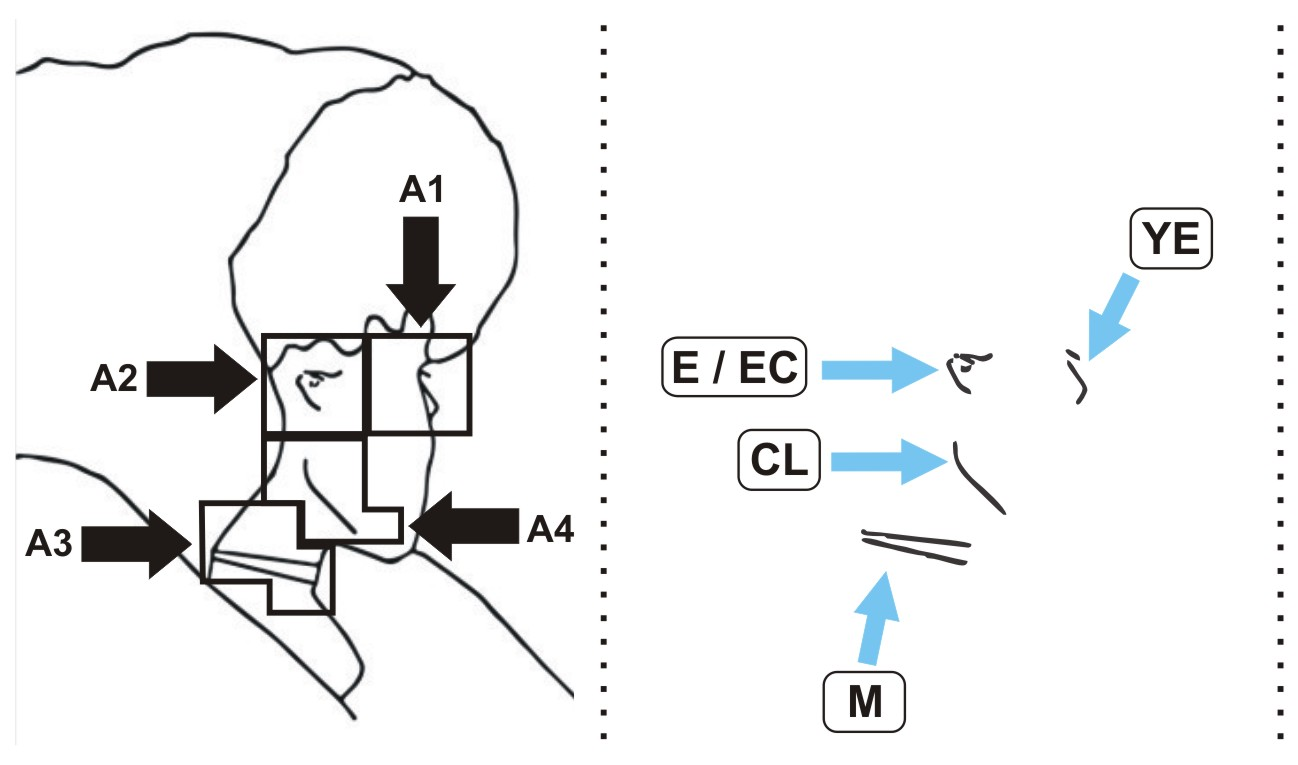
\includegraphics[width=\linewidth]{Fig1.jpeg}
    \caption{Líneas y trazos que favorecen la configuración perceptual de la imagen biestable My girlfriend or my mother-in-law. A la derecha, se aprecian los trazos establecidos por \textcite{groner_eye-movement_1983}, definiendo cuatro rasgos de modulación bottom-up: el trazo “M” favorece al percepto mujer anciana, en tanto que el rasgo YE abona en la interpretación de la mujer joven. Los trazos “E”, “EC” Y “CL” no modulan de manera específica a un percepto en particular.}
    \label{fig1}
    \source{adaptado de \textcite{groner_eye-movement_1983}}
\end{minipage}
\end{figure}

\textcite{hsiao_assessing_2012} tuvieron en cuenta estos hallazgos y, habiendo identificado y manipulado experimentalmente esos puntos de fijación moduladores de la percepción, concluyeron que lo que percibe un observador está condicionado por modulaciones de tipo \textit{bottom-up}, dadas, o bien por puntos de fijación previos a la observación de la imagen objeto de estudio, o bien por sus características físicas \cite{chastain_first_1975}, y/o por la manera en que se da la observación, dependiendo de la posición de los órganos receptores con respecto al estímulo visual \cite{polgari_novel_2020}. Estos hallazgos fueron refrendados por varios estudios centrados en analizar el efecto de congruencia semántica, valiéndose de la imagen biestable de \textcite{boring_new_1930}, donde audios coherentes semánticamente con los posibles perceptos de la imagen biestable fueron expuestos para analizar su efecto modulador \cite{hsiao_assessing_2012,marroquin-ciendua_modulacion_2020,rodriguez-martinez_ocular_2021}. En esos estudios, se confirmó la relevancia que tienen las áreas de fijación ocular en lo que respecta a la interpretación de una imagen biestable, así esté presente una estimulación auditiva en simultánea. Tanto en esos estudios, como en la investigación realizada por \textcite{hsiao_assessing_2012}, previo a la exposición del estímulo visual biestable los participantes pudieron observar un punto de fijación inicial para efectos de controlar el lugar de inicio de la observación, esto es, la primera fijación ocular.

Un punto de fijación, usado intencionalmente en tareas experimentales controladas, es un estímulo visual de entre uno y dos milímetros cuadrados que normalmente se presenta en la pantalla del dispositivo \textit{eye-tracker} (fijo) en un intervalo de entre 200 a 250 ms. (e.g. \textcite{hsiao_assessing_2012,marroquin-ciendua_modulacion_2020,rodriguez-martinez_ocular_2021}). Este punto se utiliza para direccionar la atención, como se acotó con anterioridad, para efectos de controlar el lugar en el que el participante va a iniciar su proceso de observación visual. Así, antes de una tarea experimental visual, es recomendable iniciar con un primer movimiento sacádico hacia el punto de fijación, previo a la exposición del estímulo objeto de estudio, buscando optimizar la tarea experimental desde la eliminación del sesgo definido por el lugar por donde inician las fijaciones oculares \cite{hornof_cleaning_2002}. De otra parte, el efecto modulador de las áreas de fijación ocular sobre la percepción de logotipos biestables también ha sido objeto de estudio (e.g. \textcite{rodriguez-martinez_can_2024}), hecho que permite entrever que las investigaciones fundamentadas en la psicología de la percepción visual pueden tener una aplicabilidad en dominios como la publicidad o el diseño gráfico de identificadores de marca.

Haciendo referencia a la implicación de la tecnología de registro de movimientos oculares (\textit{eye-tracking}), debe ser estimado que el estímulo a presentarse debe quedar frente a los ojos de los observadores a una distancia tal que el monitor del dispositivo quede dentro del campo visual, evitando que elementos circundantes a la pantalla puedan intervenir, por lo que suele recomendarse una distancia que, para dispositivos eye-tracker fijos de tecnología Tobii® referencia \textit{T-60} y \textit{T-120}, esté por el orden de los 60 cm. \cite{marroquin-ciendua_modulacion_2020}. En ese sentido, emergen dos planos a considerar a nivel de las pruebas experimentales, a saber, el plano de los ojos de los observadores y el plano de la pantalla de rayos infrarrojos del dispositivo \textit{eye-tracker}. Como se aprecia en la \Cref{fig2}, al plano del ojo le corresponde una referencia definida por el \textit{plano de Listing}, que es la referencia planométrica base para el registro de los movimientos oculares \cite{arango_contaminacion_2021}, en cuanto a su direccionamiento en función de los ejes “X” (eje horizontal por el que se definen los movimientos de arriba a abajo), “Y” (eje frontal por el que se establecen niveles de paralelismo entre ojo y superficie observada), y “Z” (eje vertical que define los movimientos de derecha a izquierda o viceversa). La convergencia de estos tres ejes es, sin más, el centro de rotación del ojo \cite{furman_orientation_2003}. Los movimientos y disposiciones del ojo frente a lo observado determinan las fijaciones oculares y los movimientos sacádicos manifestados durante la observación de la imagen objeto de estudio \cite{rosa_what_2015}.

Así, para el caso de estudios relacionados con comunicación de marca donde identificadores visuales o logotipos son expuestos en el monitor de aparatos fijos de registro de actividad oculomotora, se tiene que el dispositivo registrará los lugares donde hubo fijaciones oculares (coordenadas y duración), lo mismo que los trayectos recorridos por los ojos entre fijación y fijación, denominados movimientos sacádicos o sacadas \cite{ross_changes_2001}. Dado que el cerebro no procesa información visual mientras hay movimientos sacádicos \cite{rosa_what_2015}, son las fijaciones oculares y sus duraciones las que contribuyen al entendimiento de la comunicación de marca mediante el uso de logotipos biestables, cuando se desea establecer el efecto perceptual de áreas críticas de modulación \textit{bottom-up} \cite{rodriguez-martinez_can_2024}. De esta manera, hace emergencia la relación entre tecnología y comunicación, donde los sistemas de detección de movimientos basados en reconocimiento de actividad oculomotora permiten profundizar en el entendimiento de los mecanismos perceptuales implicados en la decodificación de propuestas gráficas de comunicación de marca \cite{azmy_eye_2023}. Entre más hercios (\textit{Hz.}) tenga el dispositivo, mayor es la capacidad de registro de fijaciones oculares y sacadas: si el dispositivo es de 60 \textit{Hz.}, este hará un registro de los movimientos oculares a una tasa de 60 barridas por segundo; si es de 120 \textit{Hz.}, la lectura será tomada a razón de 120 registros por segundo. Habrá, por tanto, mayor calidad de registro a mayor cantidad de hercios en el registro de la actividad oculomotora \cite{rosa_what_2015}. Como se reseñará en párrafos posteriores, el estudio que se documenta en el presente artículo utilizó un dispositivo \textit{eye-tracker} remoto de referencia Tobii® T-120. 

\begin{figure}
\centering
\begin{minipage}{.85\textwidth}
    \centering
    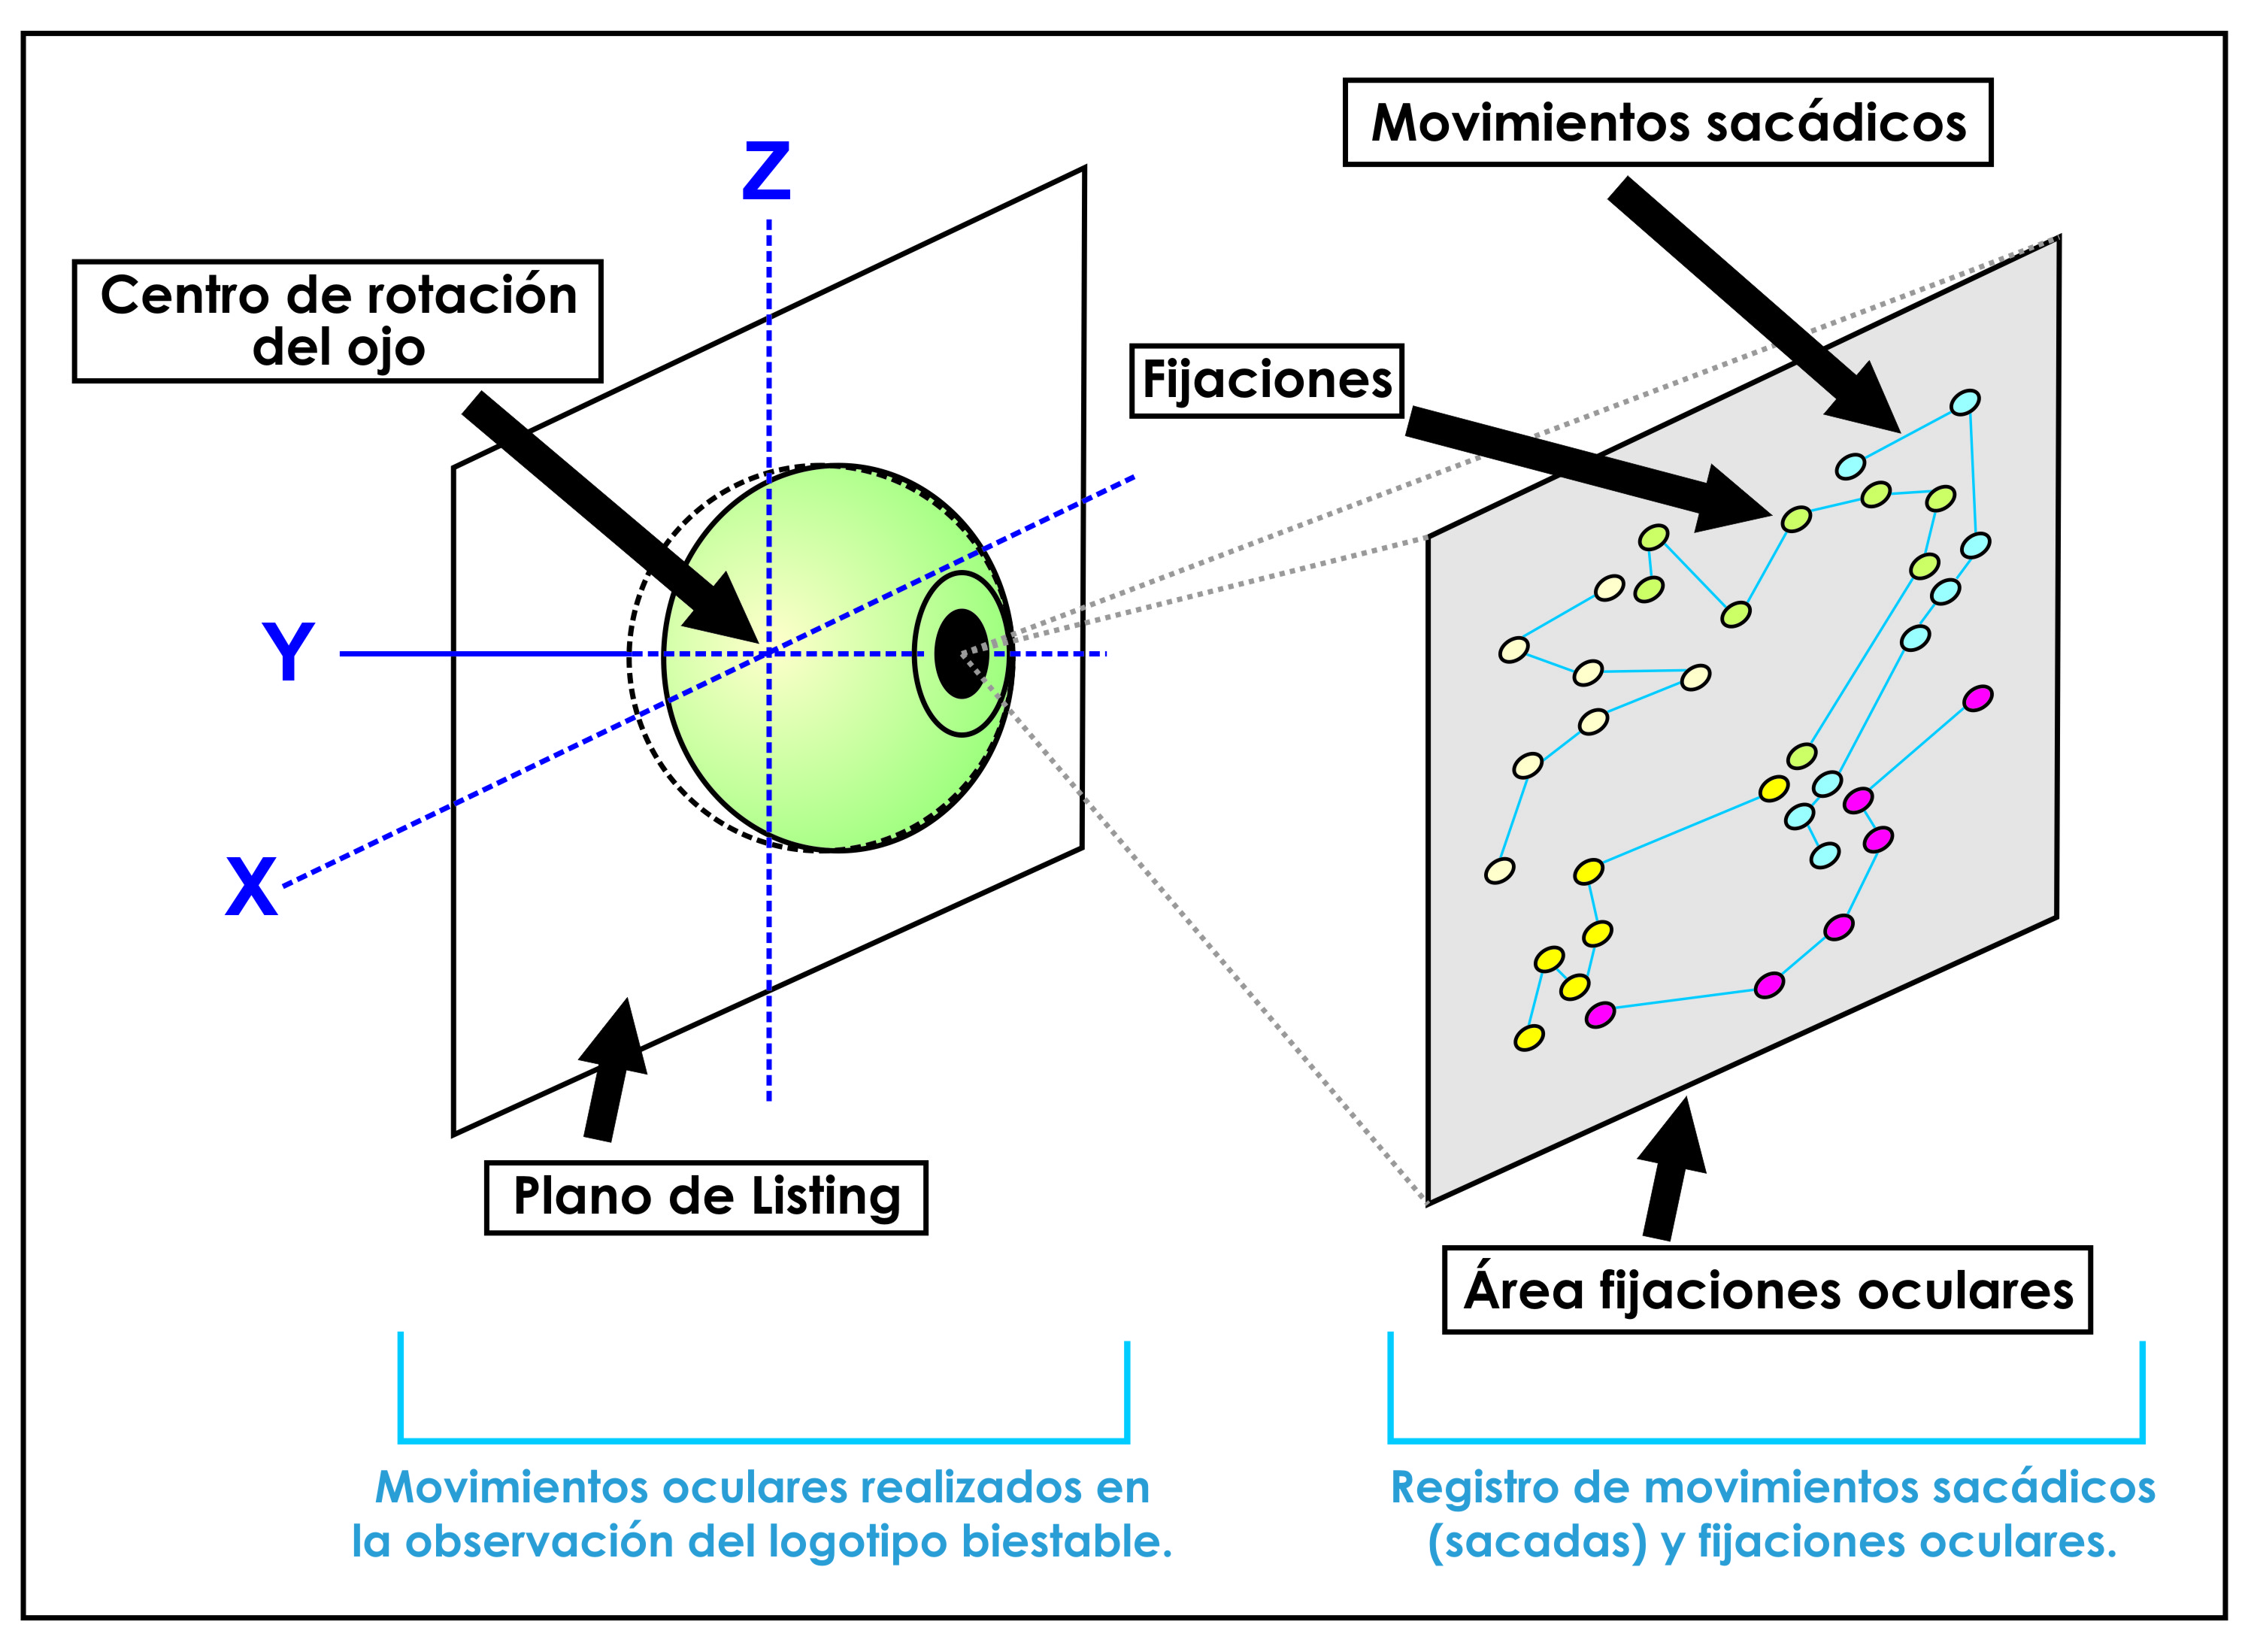
\includegraphics[width=\linewidth]{Fig2.jpeg}
    \caption{El plano de Listing y los ejes de rotación ocular (a la izquierda). En correspondencia con los movimientos oculares, en el plano de la pantalla del dispositivo eye-tracker fijo (a la derecha) se capturan las fijaciones oculares en número y duración, lo mismo que los movimientos sacádicos.}
    \label{fig2}
    \source{diseño propio.}
\end{minipage}
\end{figure}

Diversos estudios basados en registros de actividad oculomotora se han realizado con el ánimo de observar patrones de observación en marcas y logotipos biestables. \textcite{girisken_how_2014} dirimieron que existen aspectos de modulación \textit{bottom-up} que inciden en la observación de logos y emblemas de marca, dependiendo de la posición en la que estos se encuentren dentro de un determinado diseño publicitario. Por su parte, \textcite{puskarevic_eye_2016}, valiéndose de tecnología \textit{eye-tracking}, contrastaron los efectos atencionales que tienen los tipos de letra constitutivos de marcas dentro de anuncios publicitarios. Las medidas de actividad oculomotora referidas a fijaciones oculares evidenciaron la manifestación de los efectos moduladores de tipo \textit{bottom-up}, especialmente cuando las marcas apelaban a un lenguaje retórico en conjunción con tipologías de letra de mayor carga atencional. La saliencia atencional, marcada de manera importante por factores como el tamaño y los contrastes entre las formas visuales, determina, en buen grado, lo observado por los consumidores en etiquetas y diseños donde las marcas hacen presencia para diferenciarse de productos competidores, justo como lo señalan \textcite{peschel_increasing_2019}, tras haber realizado una investigación basada en registros de actividad oculomotora. En relación a estudios que en concreto han utilizado el dispositivo remoto Tobii® de referencia T-120, se encuentran investigaciones como la adelantada por \textcite{marroquin-ciendua_modulacion_2020}, o las realizadas por \textcite{rodriguez-martinez_ocular_2021,rodriguez-martinez_biestabilidad_2022}, donde el propósito esencial fue establecer áreas de modulación \textit{bottom-up} en una imagen biestable, considerando variables como las modulaciones de tipo top-down o las posiciones corporales del observador en relación a la imagen biestable presentada. Valiéndose del \textit{eye-tracker} T-120, fue posible reconocer el efecto modulador de ciertas áreas específicas del estímulo, tomando de base las duraciones de las fijaciones oculares en zonas críticas de modulación \textit{bottom-up}, áreas que, al ser observadas, generaron un efecto en la percepción final de la imagen ambigua. Para el caso concreto de investigaciones sobre logotipos biestables que instrumentalmente utilizaron el \textit{eye-tracker} T-120 de Tobii®, se tiene el estudio realizado por \textcite{rodriguez_bottom-up_2019}, donde se demostró que la colocación de puntos de fijación que orientan la mirada hacia áreas de modulación \textit{bottom-up} incide en la desambiguación de los logotipos biestables. Los análisis de las fijaciones oculares realizadas en las áreas moduladas atencionalmente por los puntos de fijación fueron el fundamento para concluir que las zonas observadas de un logotipo biestable inciden en la percepción final que se haga de él. Por su parte, \textcite{rodriguez-martinez_can_2024} logró demostrar que áreas críticas de modulación \textit{bottom-up} ejercen una influencia significativa en la percepción de un logotipo biestable. Ese estudio definió las áreas de modulación sobre la base de una cuadrícula con la cual poder determinar zonas de alta influencia perceptual, en consonancia con los aportes dados por \textcite{bernal_robayo_alisis_2020}. Los movimientos sacádicos y las fijaciones oculares fueron debidamente registradas, valiéndose del dispositivo Tobii® T-120. La tecnología del dispositivo es lo suficientemente robusta para efectos de realizar estudios centrados en la determinación de áreas de interés que sean fijadas ocularmente y que influencien la percepción de imágenes de marca de naturaleza biestable.

Debe también considerarse que, en el contexto de la comunicación de marca, son las empresas y los anunciantes quienes, en general, sugieren cuál puede ser el diseño más apropiado para sus logotipos. Cada logo tiene su propia carga de significado, pero, para el caso de identificadores visuales de tipo biestable, se reconoce que dos perceptos distintos con cargas semánticas diferentes pueden ser interpretados perceptualmente de manera diferente, donde por cada percepto se corresponde una carga semántica distinta \cite{bernal_robayo_alisis_2020,rodriguez-martinez_can_2024}. Dado que el observador puede hacer reversibilidades perceptuales, se hace manifiesta la percepción biestable, hecho que conlleva a construir, en términos perceptuales, dos distintas \textit{gestalts} \cite{de-wit_bistable_2012}, pero en momentos distintos, donde la alternancia entre cada configuración perceptual puede estar condicionada, como se ha mencionado, por las áreas del estímulo biestable que estén siendo observadas \cite{myers_ambiguous_2022}. En la \Cref{fig3} se representa el mecanismo implicado en la comunicación de marca, en función del uso de logotipos biestables, tomando en consideración que las fijaciones oculares pueden condicionar el proceso perceptual.

\begin{figure}
\centering
\begin{minipage}{.75\textwidth}
    \centering
    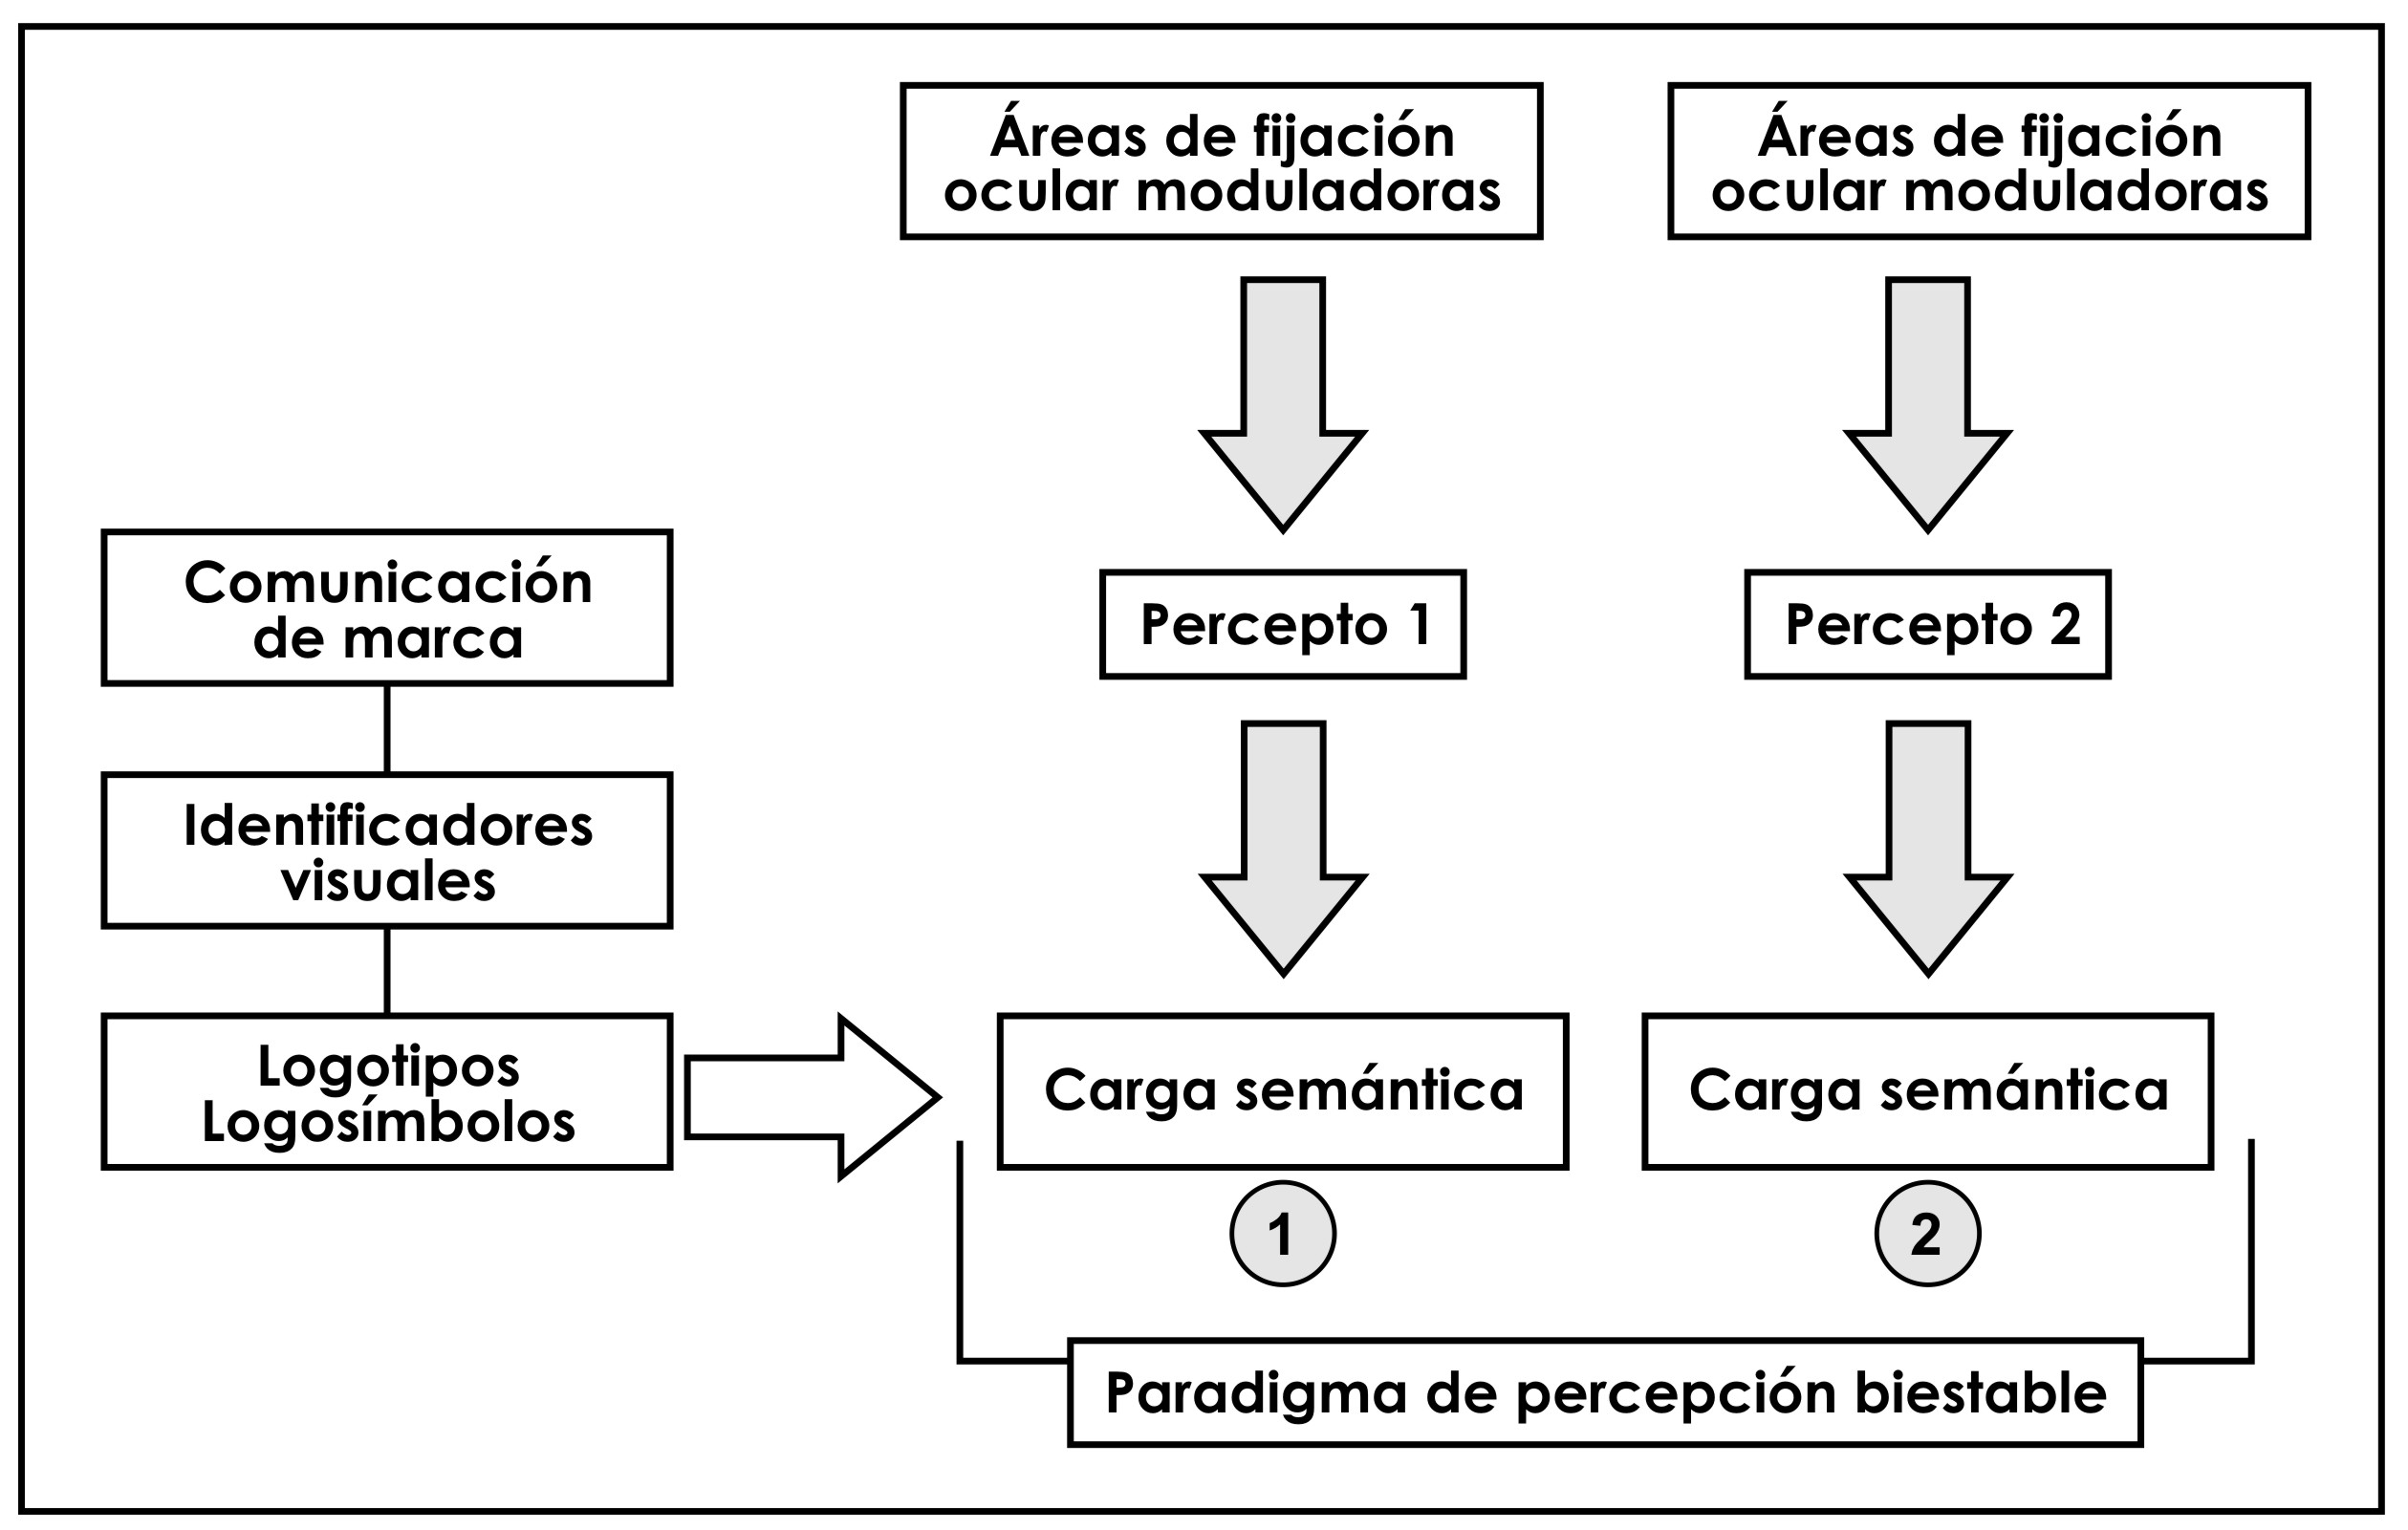
\includegraphics[width=\linewidth]{Fig3.jpeg}
    \caption{Diagrama en el cual se representa la comunicación de marca derivada de la lectura de logotipos, donde el emisor puede transmitir dos cargas semánticas diferentes al apelar a diseños basados en el paradigma de la percepción biestable.}
    \label{fig3}
    \source{diseño propio.}
\end{minipage}
\end{figure}

El estudio que acá se documenta tuvo por propósito determinar si las fijaciones oculares realizadas sobre áreas críticas de modulación \textit{bottom-up} de un logotipo biestable inciden en la configuración final de los perceptos visuales. Se planteó la hipótesis de que los perceptos reportados tendrían correspondencia con duraciones más largas de las fijaciones oculares en las áreas moduladoras con respecto a los tiempos de las fijaciones manifestadas en áreas que no se relacionan con los perceptos del logotipo biestable. Dicho de otra manera, se quiso establecer el efecto modulador de las fijaciones oculares sobre la interpretación de un identificador de marca biestable, asumiendo que a mayor tiempo se vea un área moduladora mayor probabilidad habrá de que el percepto identificado sea aquel que se relaciona con la zona de fijación moduladora. Todos los protocolos, consentimientos informados, aplicación de los mismos, más el diseño experimental y su ejecución, fueron aprobados y supervisados por el comité de ética para la investigación científica de la Universidad de Bogotá Jorge Tadeo Lozano.

\section{Metodología}\label{sec-normas}
\subsection{Diseño}

Se diseñó una tarea visual consistente en observar durante treinta segundos el logotipo de la marca colombiana de leche La Alquería®, frente a un dispositivo de registro de actividad oculomotora. Este logo se seleccionó por ser una imagen biestable que acepta dos posibles interpretaciones: una cabeza de una vaca o un chorro de leche (ver \Cref{fig4}). Se utilizó una versión simplificada del logo (trazo en línea), siguiendo el procedimiento utilizado por \textcite{groner_eye-movement_1983,marroquin-ciendua_modulacion_2020,rodriguez-martinez_can_2024}, por el cual se eliminan los rellenos y áreas con colores, lo mismo que texturas y gradaciones. Apelando a un diseño experimental, se quiso establecer si existía una relación entre las fijaciones oculares realizadas en áreas de modulación \textit{bottom-up} y los perceptos visuales identificados (cabeza de vaca o chorro de leche). Se partió de la hipótesis de que las duraciones de las fijaciones oculares registradas cuando los observadores reportan el reconocimiento de cada percepto serían mayores en las áreas críticas de modulación \textit{bottom-up} favorecedoras del percepto reportado que en las áreas que no ejercen modulación sobre él. Un punto de fijación inicial fue colocado en pantalla 250 ms. antes de la exposición del logo, justo en el área inferior, centrado, esto para eliminar el sesgo de la primera fijación ocular (para todos los participantes la primera observación estaría condicionada por el enganche atencional de ese punto). En la \Cref{fig4} se aprecia la colocación del punto de fijación con relación a la posterior exhibición del logo en línea.

\begin{figure}
\centering
\begin{minipage}{.75\textwidth}
    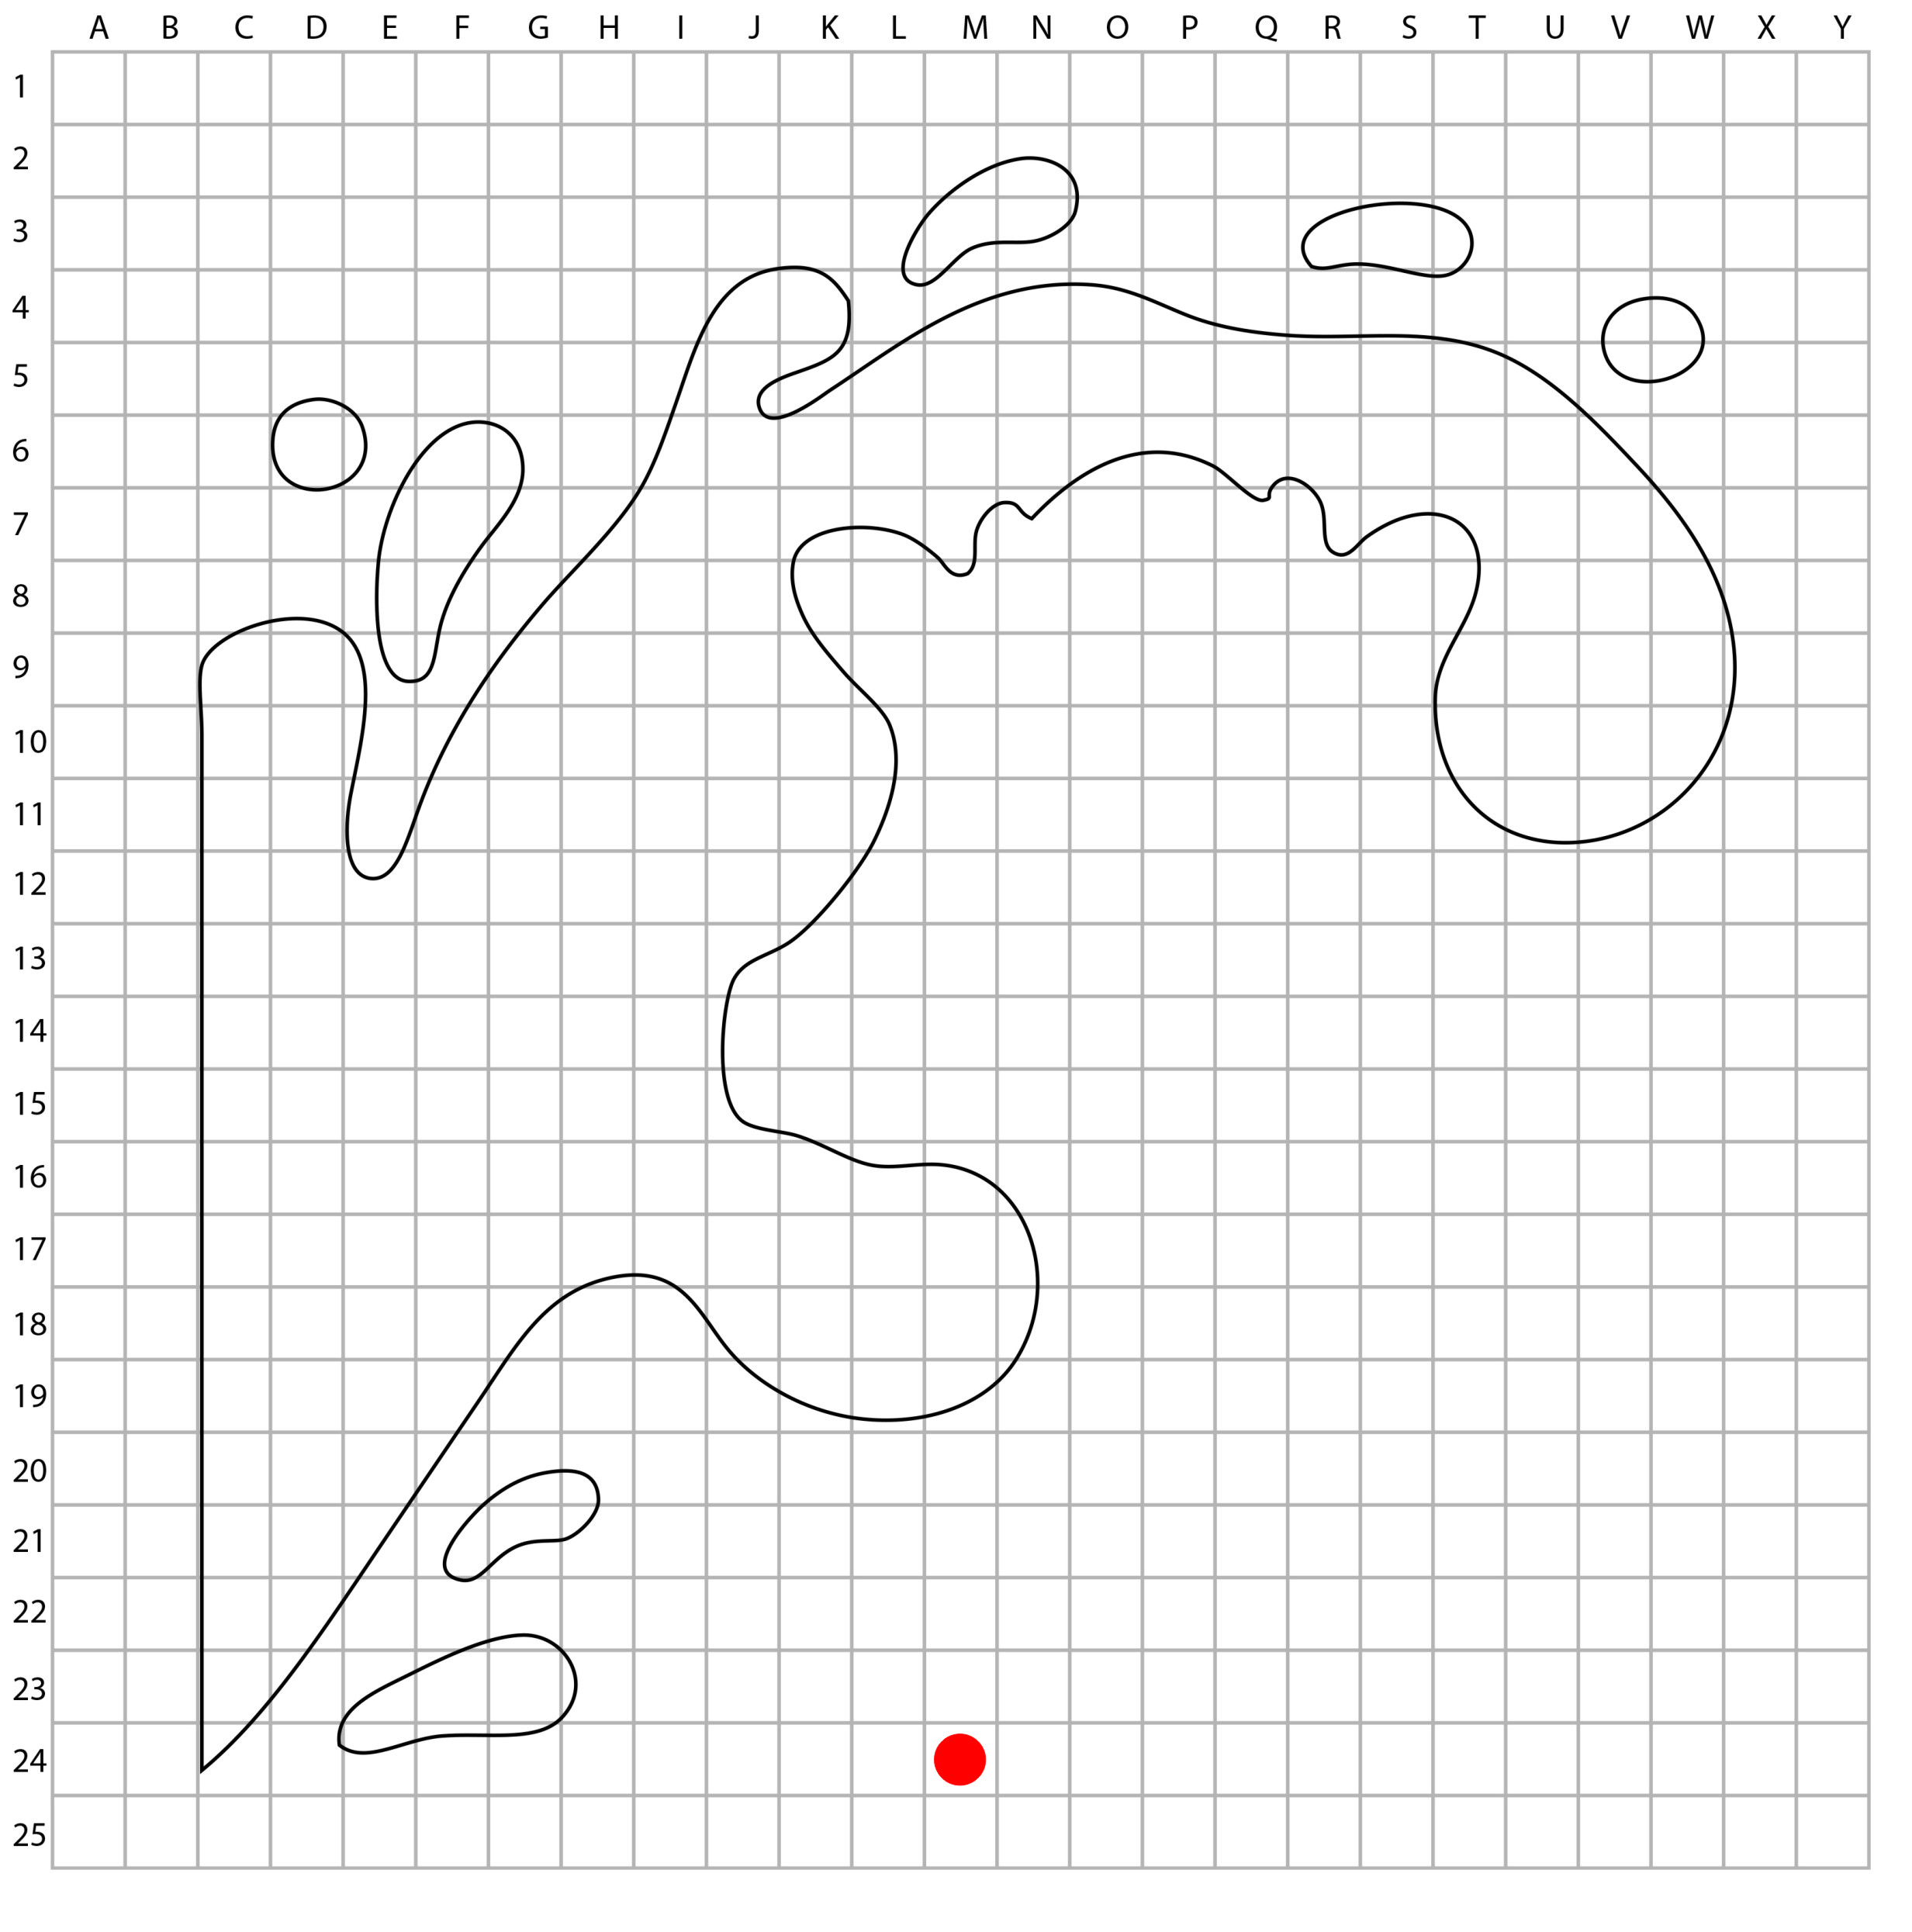
\includegraphics[width=\linewidth]{Fig4.jpeg}
    \caption{Logotipo biestable utilizado en la prueba experimental. El logo biestable fue llevado a trazos de línea, siguiendo parámetros metodológicos considerados por \textcite{groner_eye-movement_1983,marroquin-ciendua_modulacion_2020,rodriguez-martinez_can_2024}. Abajo, en el centro, se aprecia (en rojo) la colocación del punto de fijación inicial.}
    \label{fig4}
    \source{diseño propio.}
\end{minipage}
\end{figure}

\subsection{Participantes}\label{sec-conduta}

Veinticinco voluntarios participaron en este estudio (44\% hombres, 56\% mujeres; rango de edad entre 21 y 28 años; $M = 24.32$; $D.E. = 2.13$). Todos los participantes desconocían el propósito del estudio y tenían una visión normal o corregida (mediante lentes de contacto). Cada uno de ellos proporcionó su consentimiento informado por escrito. La tarea visual se llevó a cabo en una cámara experimental en un laboratorio de psicología experimental. Los participantes se seleccionaron de conformidad con una prueba de cribado obtenida mediante \textit{sub-tests} perceptuales y cognitivos aplicados previamente. Los veinticinco participantes obtuvieron en las evaluaciones de sus pruebas de cribado una puntuación que implicó normalidad en términos de desempeño cognitivo y perceptual.

\subsection{Aparatos y materiales}\label{sec-fmt-manuscrito}
Para efectos de realizar tamizajes perceptuales y cognitivos con los cuales garantizar el estado mental y físico óptimo de los participantes para realizar la tarea experimental, se aplicó, en primera instancia, el sub-test breve para la evaluación del estado cognitivo (BCSE), instrumento de aplicación individual diseñado para evaluar brevemente el funcionamiento cognitivo general en adultos y que se utilizó en el estudio para efectos de seleccionar la muestra. Fue seleccionado este sub-test dado que con él se pueden evaluar déficits de memoria o trastornos neurológicos, psiquiátricos o del desarrollo, siendo muy válido para observar desempeños de aprendizaje y evocación \cite{chirivella_test_2003}. Este sub-test hace parte de la Escala de Memoria de Wechsler (IV), que es una escala de aplicación individual que evalúa diferentes capacidades mnésicas. Posteriormente, se aplicó a los participantes el sub-test 1 y 4 (de \textit{Discriminación Visual} y de \textit{Cierre Visual}, respectivamente), pertenecientes al test de Percepción Visual no Motriz [TPVNM], cuyo propósito consiste en evaluar el funcionamiento perceptual visual mediante tareas de rápida aplicación e interpretación \cite{merino_test_2008}.

El primer sub-test (de \textit{Discriminación Visual}), se seleccionó en razón a que la tarea propia del estudio implicaba una discriminación visual en el sentido de distinguir una u otra imagen posible entre las dos posibles interpretaciones del estímulo visual biestable. En efecto, con este sub-test se evalúa esa capacidad de reconocimiento de estímulos visuales entre un conjunto, reconocimiento implicado durante la percepción de figuras ambiguas \cite{rock_why_1994}. Como complemento, se incorporó el cuarto sub-test del test TPVNM, referido a la valoración de la capacidad de hacer cierres perceptuales. Este test se consideró útil para el cribado de los participantes, en cuanto a que la capacidad de hacer cierres perceptuales está involucrada en el proceso de desambiguación perceptual de los estímulos biestables \cite{pressnitzer_temporal_2006}. Una vez los participantes aprobaron las pruebas de tamizaje, procedieron a hacer la prueba como tal. Para ese propósito, se utilizó, como se mencionó con anterioridad, un dispositivo \textit{eye-tracker} fijo de 120 Hz., tecnología Tobii®, referencia T-120. El estímulo visual fue presentado en ese dispositivo para así poder obtener todos los registros de actividad oculomotora, fijaciones oculares, movimientos sacádicos y duraciones de cada fijación ocular manifestada en las áreas de modulación \textit{bottom-up}, tal y como se reseñará más adelante, en el apartado \textit{procedimiento}. El \textit{eye-tracker} utilizado fue diseñado por la compañía sueca Tobii AB. Con una tasa de refrescamiento de 120 Hz., el dispositivo toma 120 registros por segundo \cite{tobii_ab_user_2012}, lo que le permite ser óptimo para investigación en lo relativo a tareas visuales centradas en análisis de áreas de interés, basándose en registros de fijaciones oculares y movimientos sacádicos \cite{hahn_eye_2022}.

Cuando se usa el dispositivo T-120, la recomendación es diseñar experimentos en los que los participantes mantengan firme su posición durante las pruebas respectivas, esto porque es un aparato que puede perder muchos registros como consecuencia de desviaciones en la orientación de la cabeza \cite{hessels_qualitative_2015}. No obstante, este \textit{eye-tracker} tiene la capacidad de registrar los movimientos oculares cuando se presentan leves movimientos de la cabeza durante las tareas experimentales \cite{leckey_response_2020}. La luminiscencia del monitor del aparato cumple con la norma europea IEC/EN 60825-1/A1-A2, clase 1, para productos LED destinados a tener exposiciones prolongadas de imágenes \cite{tobii_ab_user_2012}. La norma establece un límite de emisión accesible para garantizar una exposición continua, donde el límite está dado por la iluminación máxima a la que una persona debe estar expuesta durante ocho horas al día durante varios días seguidos. Así mismo, el fabricante recomienda utilizar el dispositivo de manera tal que el observador esté a una distancia aproximada de 60 cms. A esta distancia, la exposición de luz de este \textit{eye-tracker}, promediada en tiempo, es equivalente al 0,1 \% del límite permitido para exposiciones prolongadas, según la normatividad. Esta configuración requiere de la versión Tobii Studio®, que es el software requerido para operar el dispositivo de manera remota \cite{arfe_effects_2023}. Es por esto que este tipo de dispositivos se conocen también con el nombre de \textit{remote eye-tracker devices} \cite{hessels_qualitative_2015}.


\subsection{Procedimiento}\label{sec-formato}
Cada participante observó el logotipo biestable durante 30 segundos, frente al dispositivo de registro de actividad oculomotora. La distancia que se consideró entre cada participante y el monitor fue de 60 centímetros, como se ha reportado en otros estudios (e.g. \textcite{marroquin-ciendua_modulacion_2020,rodriguez-martinez_biestabilidad_2022} y como sugiere el fabricante del dispositivo utilizado. A todos los sujetos se les dio la instrucción de mantener la cabeza inmóvil durante la tarea, dada la duración de la misma. Los participantes reportaron de manera oral el percepto que reconocían (cabeza de vaca/chorro de leche). Se instruyó también a los participantes sobre el hecho de oprimir el botón izquierdo de un \textit{mouse} de computador cada vez que reconocían uno u otro percepto. De esta manera, se capturó el momento del reconocimiento de cada percepto, mientras que el establecimiento del percepto particularmente identificado se dio por la palabra usada en correspondencia con este (“cabeza” si lo reconocido era la cabeza de la vaca, percepto “V”; “chorro de leche”, si lo reconocido era el chorro de leche, percepto “C”). Este paradigma procedimental fue definido en consonancia con el estudio realizado por \textcite{rodriguez-martinez_ocular_2021} y estimando áreas de modulación \textit{bottom-up} según los reportes realizados por \textcite{rodriguez-martinez_can_2024}.

Los datos recogidos fueron organizados en una hoja de cálculo, discriminados por las duraciones de las fijaciones oculares y por las áreas observadas, en consideración a los perceptos V y C. 12 áreas de modulación \textit{bottom-up} fueron consideradas en el estudio, 6 referidas a la percepción de la cabeza de vaca (áreas A1, A2, A3, A4, A5 y A6), y otras 6 correspondientes a zonas que influencian el reconocimiento del chorro de leche (A7, A8, A9, A10, A11 y A12), como se muestra en la \Cref{fig5}. Cada una de estas zonas de fijación ocular contaron con la misma área (en términos de milímetros cuadrados) y se definieron en relación a una cuadrícula general, de manera tal que cada una de ellas constituyera un cuadrado definido por solo cuatro unidades cuadráticas (ver \Cref{fig5}). La definición de estas zonas, en relación con su potencial modulación de tipo \textit{bottom-up}, estuvo dada de conformidad con los hallazgos del estudio adelantado por \textcite{bernal_robayo_alisis_2020} y siguiendo procedimientos planteados por \textcite{rodriguez-martinez_can_2024}. Para comprobar la hipótesis planteada, se cotejaron las duraciones de las fijaciones oculares manifestadas en las áreas de modulación \textit{bottom-up} que se corresponden con cada uno de los perceptos reportados. Todos los datos se procesaron utilizando los programas Tobii Studio®, Excel® (v.16.45) y SPSS® (v.23).

\begin{figure}
\centering
\begin{minipage}{.75\textwidth}
    
\includegraphics[width=\linewidth]{Fig5.jpeg}
    \caption{Las áreas de fijación ocular definidas para el estudio. Las zonas A1, A2, A3, A4, A5 y A6 se corresponden con zonas moduladoras del percepto V (cabeza de vaca). Las áreas A7, A8, A9, A10, A11 y A12 se asocian con el percepto C (chorro de leche).}
    \label{fig5}
    \source{diseño propio.}
\end{minipage}
\end{figure}

\section{Resultados}\label{sec-modelo}
Al considerar los resultados obtenidos de los 25 participantes, se encuentra que al comparar las sumatorias de las duraciones de las fijaciones oculares del grupo de áreas observadas moduladoras del percepto V (A1, A2, A3, A4, A5 y A6) con las del grupo de áreas moduladoras del percepto C (A7, A8, A9, A10, A11 y A12), resultan ser mayores las duraciones para cuando el percepto reportado es consistente con las áreas moduladoras del caso. Dicho de otra manera, cuando se toman los reportes que se correspondieron con el percepto C donde estuvieron implicadas las observaciones en las áreas de modulación de dicho percepto, se encuentra que el promedio de las duraciones de esas fijaciones oculares ($M = 14.56$; $DE = 5.16$); $t(24) = 5.322$; $p = .000$) es significativamente mayor que el promedio de las duraciones de las fijaciones manifestadas sobre las áreas de modulación que favorecen al percepto V ($M = 7.72$; $DE = 4.22$) cuando se reporta el percepto C.

Por otra parte, los reportes referidos al percepto V en correspondencia con la observación de sus zonas moduladoras, implican una duración de las fijaciones oculares significativamente mayor ($M = 14.39$; $DE = 9.32$; $t(24) = 2.575$; $p = .008$) que el tiempo dado a las observaciones en áreas no moduladoras ($M = 7.6$; $DE = 5.49$), cuando se da ese reporte V. En la \Cref{tb1} se aprecian los valores totales de las duraciones de las fijaciones oculares considerando cada percepto identificado y la suma de las duraciones de las fijaciones oculares en las 6 áreas moduladoras de uno y otro percepto; los términos “congruente” y “no congruente” hacen alusión a si las fijaciones oculares fueron realizadas dentro de áreas de modulación congruentes o no congruentes (respectivamente) con el percepto reportado:

\begin{table}[htbp]
\centering
\begin{threeparttable}
\caption{Total de las duraciones de las fijaciones oculares considerando el percepto reportado y el total de visitas a los cuadrantes de modulación \textit{bottom-up}.}
\label{tb1}
\begin{tabular}{l l l l}
\toprule
\multicolumn{1}{>{\raggedright}p{2.5cm}}{
Percepto ``Vaca'' -- Congruente} & \multicolumn{1}{>{\raggedright}p{2.5cm}}{Percepto ``Vaca'' -- No congruente} & \multicolumn{1}{>{\raggedright}p{2.5cm}}{Percepto ``Chorro'' -- No congruente} & \multicolumn{1}{>{\raggedright}p{2.5cm}}{Percepto ``Chorro'' -- Congruente}\\ 
\midrule
5,19 & 5,11 & 5,22 & 5,13 \\ 
9,58 & 18,9 & 9,58 & 19,9 \\ 
2,75 & 10,91 & 2,98 & 15,83 \\ 
4,86 & 9,89 & 10,06 & 9,39 \\
4,56 & 10,68 & 4,56 & 13,43 \\
0,98 & 15,07 & 3,95 & 20,56 \\
20,76 & 8,99 & 11,07 & 15,72 \\
0,88 & 1,75 & 0,88 & 2,8 \\
11,33 & 10,16 & 5,3 & 10,16 \\
23,35 & 5,79 & 13,52 & 11,29 \\
14,13 & 15,72 & 4,95 & 24,47 \\
3,62 & 3,59 & 2,5 & 13,23 \\
25,72 & 3,81 & 11,84 & 10,23 \\
19,13 & 4,82 & 9,8 & 4,84 \\
19,46 & 9,59 & 12,94 & 16,67 \\
25,72 & 3,81 & 11,84 & 10,23 \\
21,85 & 1,3 & 12,98 & 16,04 \\
4,54 & 16,49 & 12,3 & 16,67 \\
18,7 & 4,26 & 3,3 & 16,87 \\
26,01 & 3,93 & 10,05 & 18,82 \\
25,72 & 1,75 & 3,3 & 16,87 \\
21,85 & 1,3 & 12,98 & 16,04 \\
4,51 & 16,46 & 12,6 & 16,64 \\
18,7 & 4,26 & 3,3 & 16,87 \\
26,04 & 3,89 & 10,08 & 18,79 \\
\bottomrule
\end{tabular}
\source{diseño propio.}
\end{threeparttable}
\end{table}

Cuando se grafican estos resultados, se puede apreciar cómo los reportes de los perceptos varían de conformidad con las áreas observadas de la imagen, notándose que se da una mayor duración de las fijaciones oculares en las áreas correspondientes a los perceptos identificados. Al observar la \cref{fig6}, se aprecia cómo los tiempos promedio de las fijaciones oculares tomados en las observaciones dadas a los grupos de áreas moduladoras son mayores cuando se da una correspondencia entre el percepto reportado y el área moduladora correspondiente a dicho percepto.

\begin{figure}[htbp]
\centering
\begin{minipage}{.75\textwidth}
    \centering
    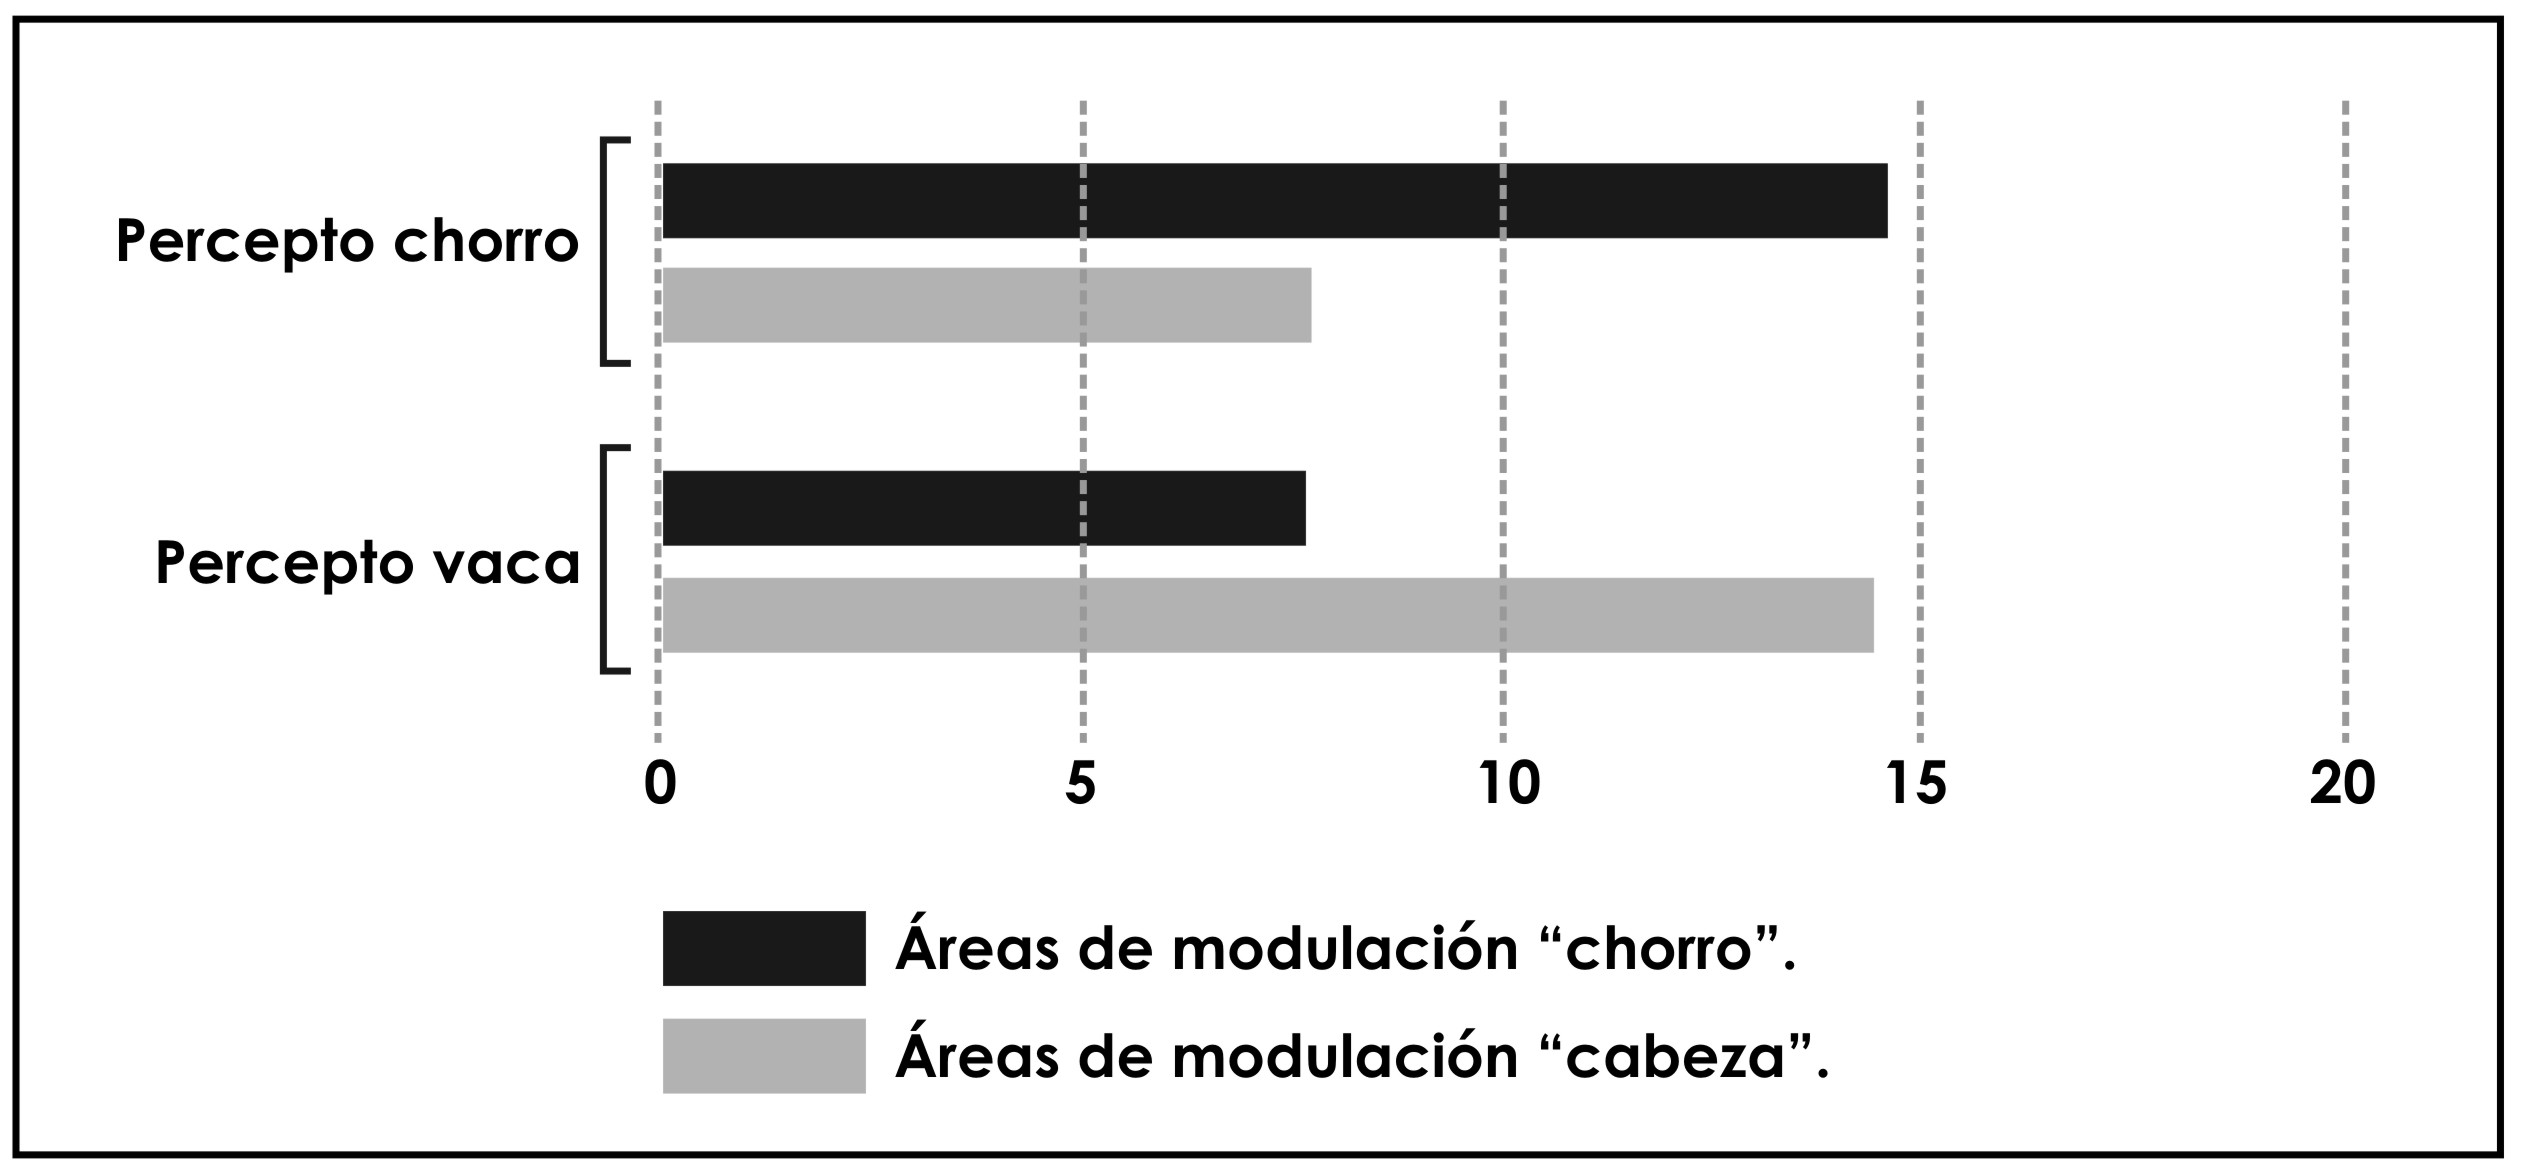
\includegraphics[width=\linewidth]{Fig6.jpeg}
    \caption{Comparación de las duraciones de las fijaciones oculares en segundos, considerando las áreas de modulación bottom-up.}
    \label{fig6}
    \source{diseño propio.}
\end{minipage}
\end{figure}

En la \Cref{fig7}, por su parte, se visibiliza el comportamiento de las duraciones de las fijaciones oculares por cada participante cuando se reporta el percepto V. En términos descriptivos se nota cómo ese percepto se reconoce mayormente cuando las fijaciones oculares recaen en las áreas moduladoras de ese percepto (A1, A2, A3, A4, A5 y A6).

\begin{figure}
\centering
\begin{minipage}{.75\textwidth}
    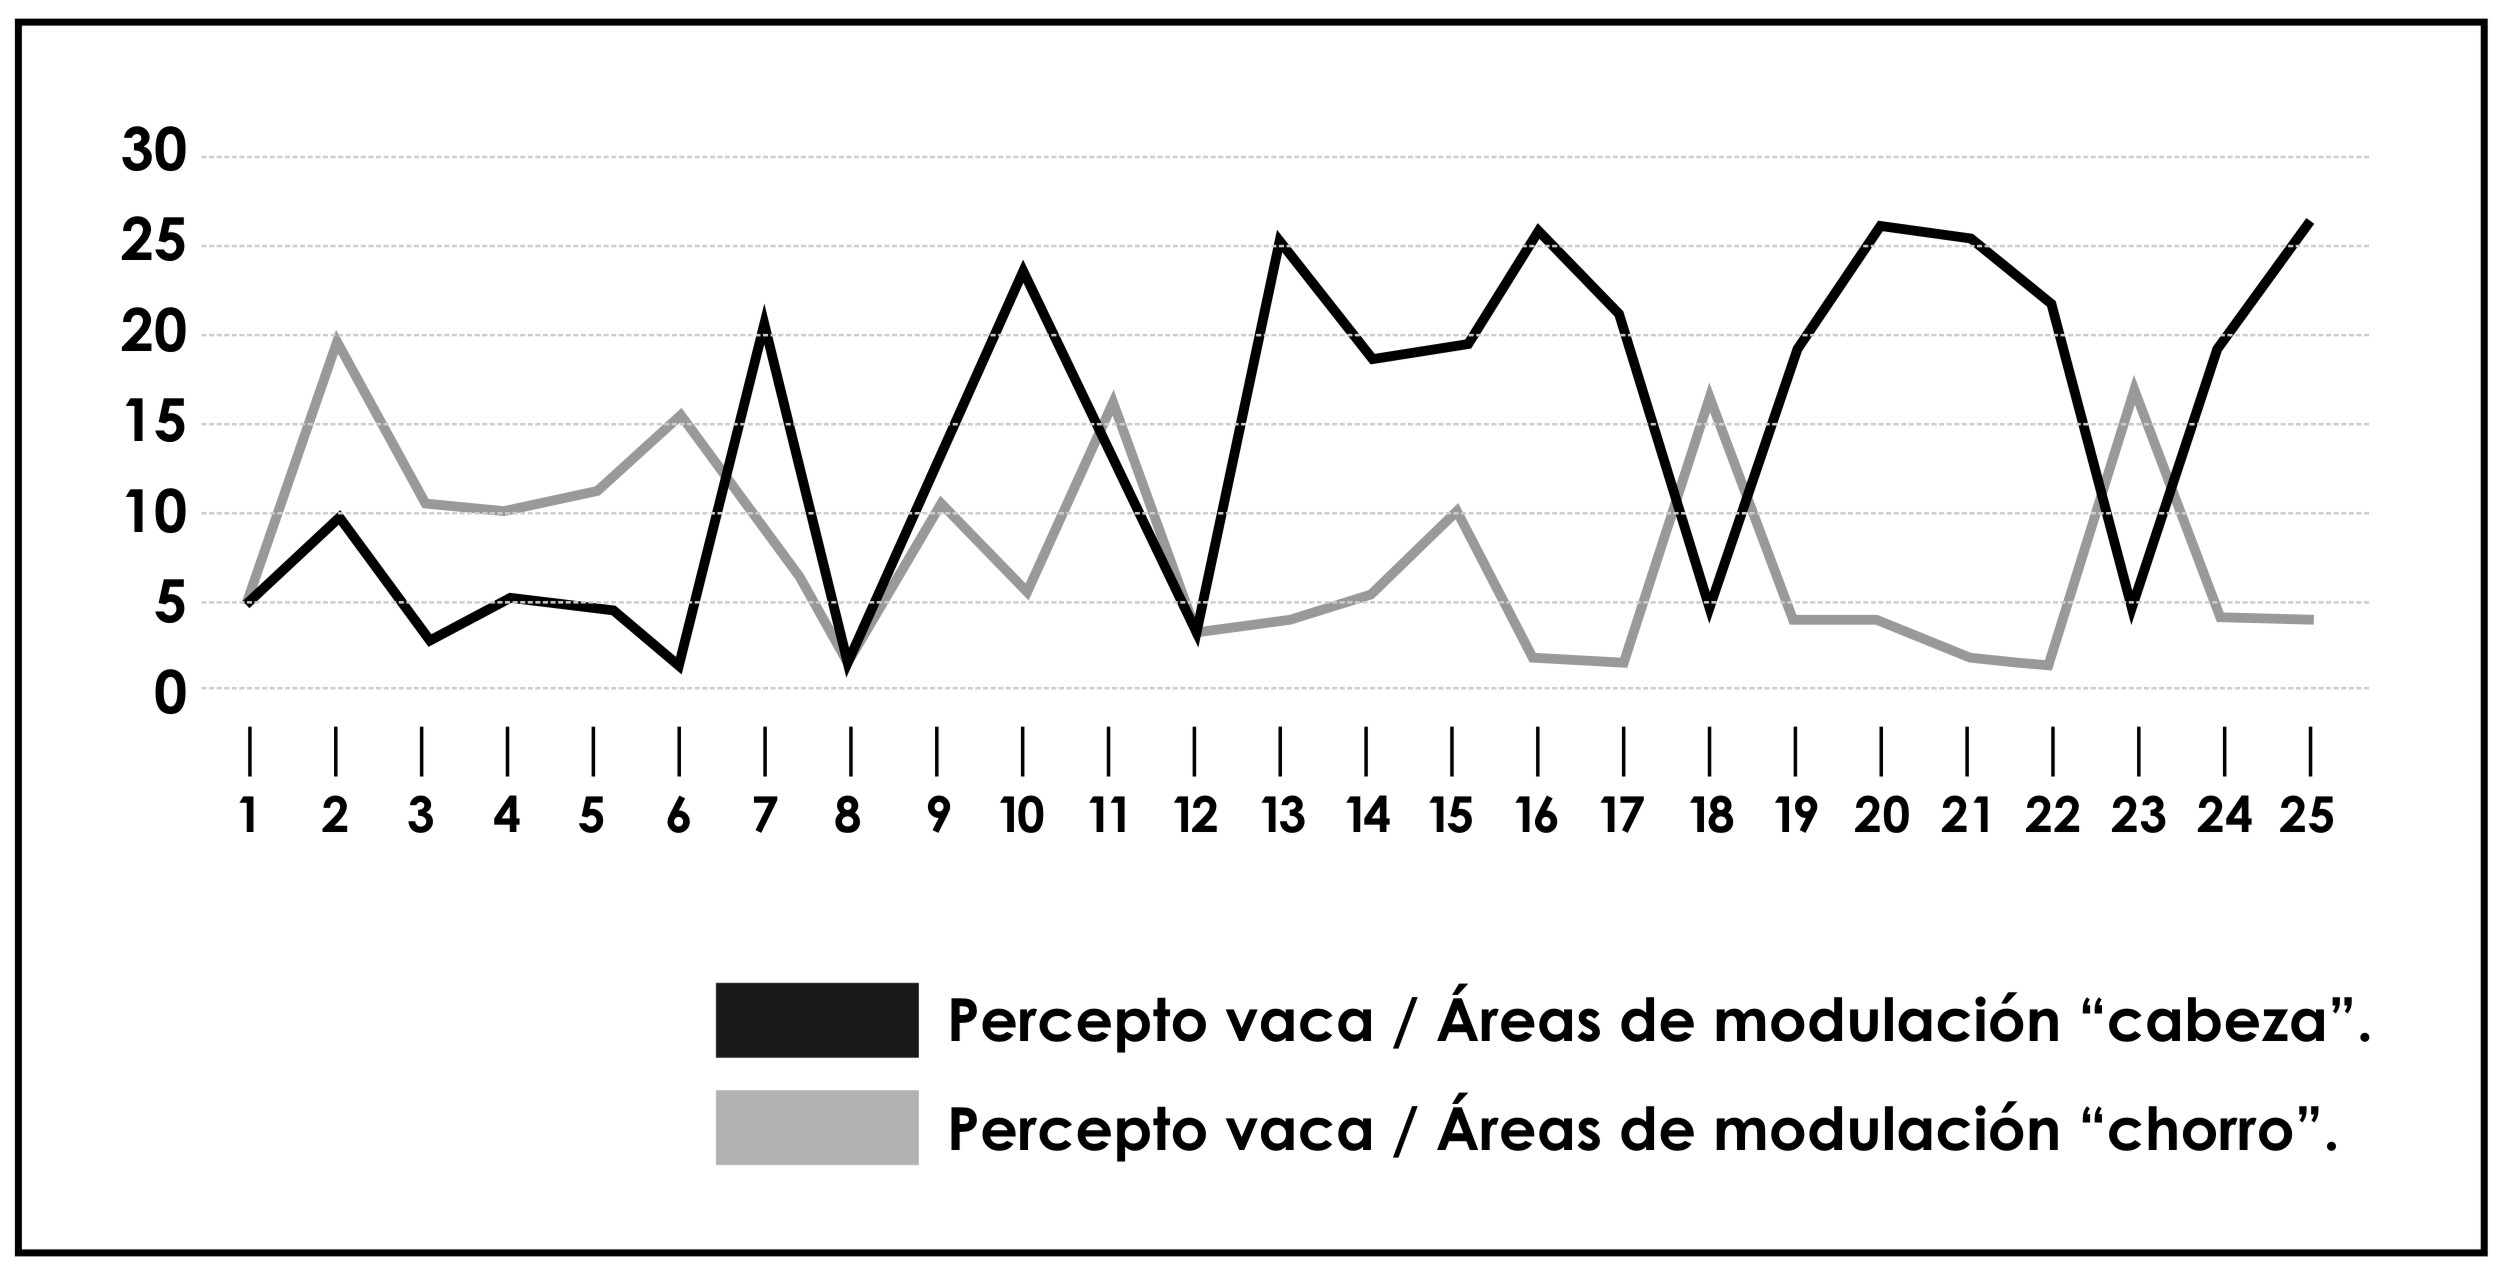
\includegraphics[width=\linewidth]{Fig7.jpeg}
    \caption{Duraciones de las fijaciones oculares en las áreas moduladoras del percepto V en relación a los reportes de los perceptos C y V. En negro, las duraciones de las fijaciones para el percepto V (vaca) en áreas moduladoras de ese percepto. En gris, las duraciones de las fijaciones para el mismo percepto reportado, pero estando el ojo en las áreas moduladoras del percepto C.}
    \label{fig7}
    \source{diseño propio.}
\end{minipage}
\end{figure}

En la \Cref{fig8}, se reconoce cómo para el reporte del percepto C se da un mayor tiempo de las fijaciones oculares en las áreas moduladoras que se corresponden a la identificación de dicho percepto (A7, A8, A9, A10, A11 y A12). Al cotejar los datos, tanto de manera descriptiva como desde los resultados obtenidos con los análisis de estadística inferencial, se reconoce que los grupos de áreas moduladoras sí ejercen un efecto, reconociéndose el potencial efecto modulador de las zonas por las que el ojo se posa, en términos de fijaciones oculares. Debe ser estimado que, cuando se realizaron los análisis, sólo fueron estimados los tiempos de fijación ocular manifestados en las áreas de análisis del caso o áreas de interés (AOIs). Las fijaciones oculares que no se correspondieron con las AOIs seleccionadas (desde A1 hasta A12) no fueron estimadas en el estudio y se catalogaron como fijaciones oculares manifestadas en un área neutra.

\begin{figure}
\centering
\begin{minipage}{.75\textwidth}
    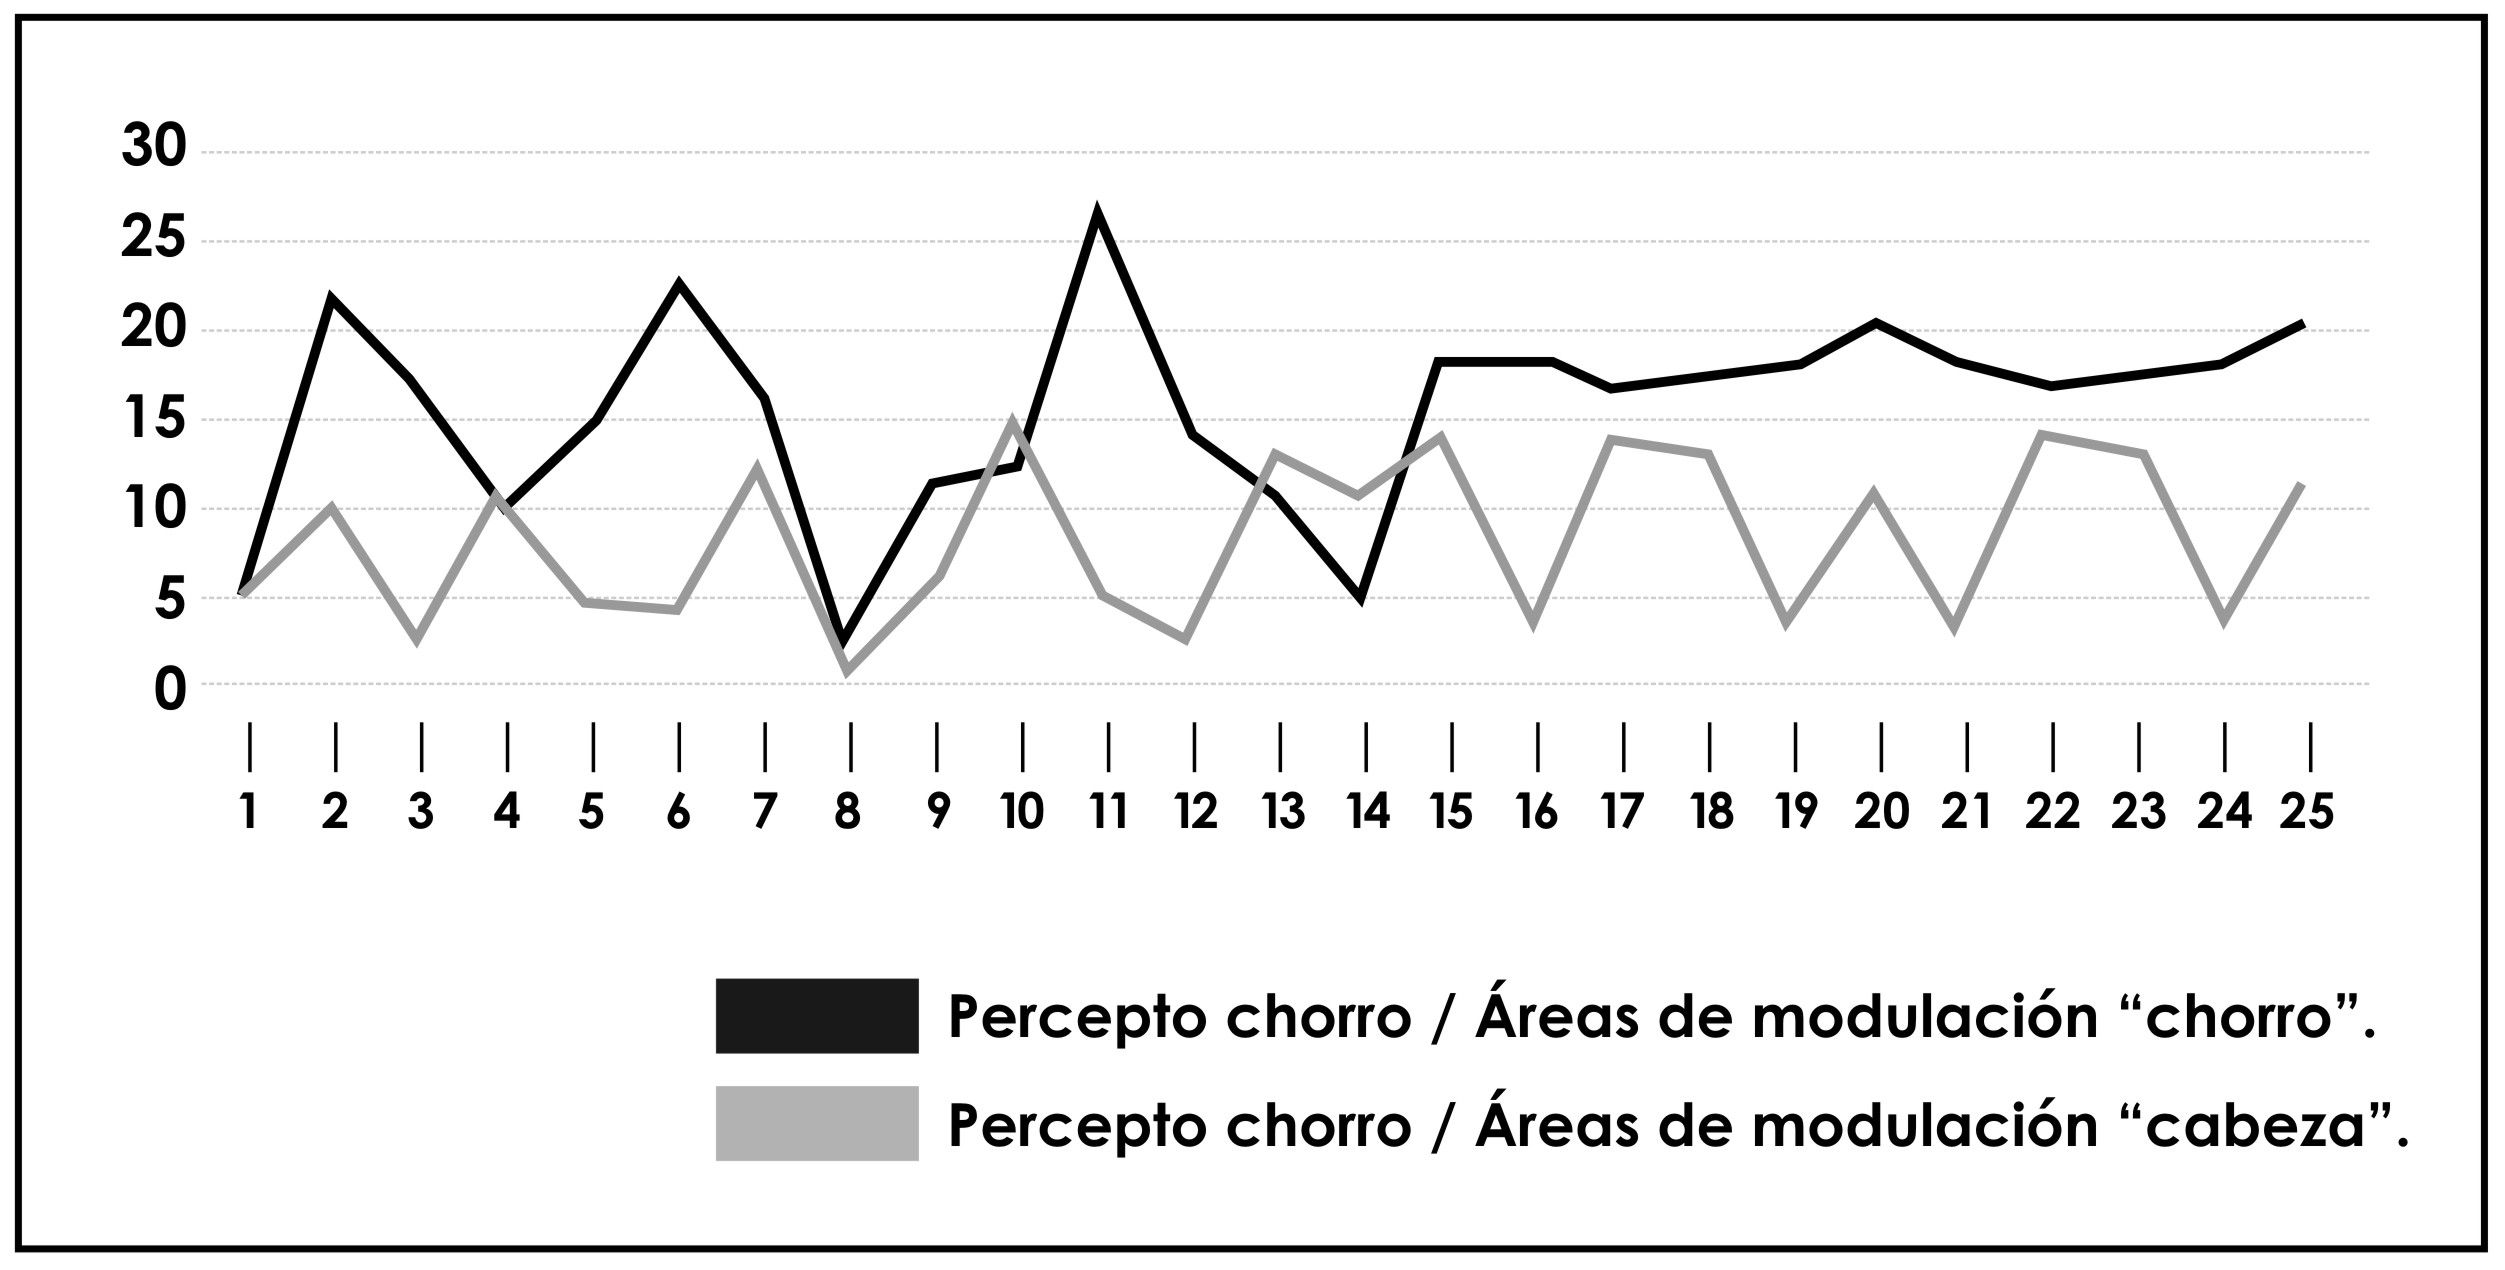
\includegraphics[width=\linewidth]{Fig8.jpeg}
    \caption{Duraciones de las fijaciones oculares en las áreas moduladoras del percepto C en relación a los reportes de los perceptos C y V. En negro, las duraciones de las fijaciones para el percepto C (chorro) en áreas moduladoras de ese percepto. En gris, las duraciones de las fijaciones para el mismo percepto reportado, pero estando el ojo en las áreas moduladoras del percepto V.}
    \label{fig8}
    \source{diseño propio.}
\end{minipage}
\end{figure}


\section{Discusión}\label{sec-organizacao}
De conformidad con los resultados, se reconoce que existe un efecto modulador de las áreas de fijación ocular sobre la configuración perceptual del logotipo biestable utilizado en la tarea experimental. Estos resultados están en línea con los hallazgos que se encuentran en los estudios de \textcite{rodriguez_bottom-up_2019} y de \textcite{rodriguez-martinez_can_2024}. Sin embargo, la investigación acá documentada toma en consideración la duración que tienen las fijaciones oculares en las correspondientes áreas de modulación, para cada posible percepto a interpretar dentro del logotipo biestable. En el estudio de \textcite{marroquin-ciendua_modulacion_2020}, si bien se estimaron duraciones en lo referente al lapso entre el reporte de un percepto y el reporte del otro percepto, no se contemplaron las duraciones que de manera específica hicieran referencia a las fijaciones oculares hechas en las áreas críticas de modulación \textit{bottom-up}.

Resulta así significativo el aporte que se da en este estudio, primero porque se analiza la relación entre las fijaciones oculares en áreas moduladoras y los perceptos que los observadores identifican, y segundo, porque pone a prueba el mecanismo de modulación de la percepción biestable, esta vez no en imágenes biestables tradicionalmente usadas en el contexto de la investigación psicológica (e.g. \textcite{rock_why_1994,kornmeier_ambiguous_2012,hsiao_assessing_2012}, sino en un identificador de marca que tiene las características propias de los estímulos visuales biestables, en línea con las aportaciones dadas por \textcite{rodriguez-martinez_can_2024}. 

Esta aplicación de los mecanismos implicados en la percepción biestable supone un aporte válido para ser considerado por parte de quienes diseñan este tipo de estímulos en el contexto de las comunicaciones de marca, justo como también se puede encontrar en varios de los resultados expuestos por \textcite{azmy_eye_2023}, y por \textcite{rodriguez-martinez_can_2024}. De manera específica, la técnica de registro de actividad oculomotora (\textit{eye-tracking}), se reivindica como una alternativa instrumental válida para desentrañar mecanismos perceptuales implicados en la relación consumidor-marca \cite{santos_eye_2015}, donde, de manera prospectiva, es visible el modo en que esta instrumentalización aporta a decisiones referidas al diseño y las comunicaciones, en función del conocimiento de los paradigmas implicados al cotejar medidas de registro de movimientos oculares \cite{rosa_what_2015}. Recuérdese que las técnicas de registro de actividad oculomotora permiten monitorear y observar los movimientos oculares mientras se mira un determinado objeto, llámese imagen estática, imagen dinámica, interfaz, etc. \cite{rosa_what_2015}. Estas técnicas, conocidas también en idioma inglés como \textit{eye-tracking techniques}, buscan comprender cómo un observador analiza y mira un determinado estímulo o conjunto de estímulos visuales \cite{fu_advances_2016}, pudiéndose tomar varias medidas una vez la data ha sido arrojada por el \textit{software} respectivo, eligiendo entre diferentes alternativas y hallando respuestas a una determinada necesidad de información \cite{carter_best_2020}. En ese sentido, es posible determinar patrones de fijación ocular, duración de las fijaciones (en unidades de milisegundos que serán mayores o menores dependiendo del dispositivo \textit{eye-tracker} en específico), desplazamientos y vectores de los movimientos sacádicos, coordenadas de cada fijación ocular, actividad de cambio en el diámetro pupilar, entre otros \cite{tien_eye_2014}. En consecuencia, si los diseñadores y comunicadores de marca deciden elaborar un estímulo visual con doble carga semántica para así abonar en la concreción de un determinado plan estratégico de marca y/o de mercadeo, y si para transmitir esos dos distintos significados se valen de identificadores visuales de naturaleza biestable, los aportes otorgados por la investigación neurocientífica ayudarían a mejorar el diseño de logotipos, si se determinan patrones de recorridos visuales y áreas de modulación que orienten la interpretación y decodificación de las cargas semánticas implicadas. Revisando los resultados del presente estudio, se advierten unas relaciones entre ciertas zonas específicas de la imagen y su respectiva interpretación. Los patrones atencionales implicados están vinculados a los tiempos de cada fijación ocular, hecho que conlleva a exponer la idea de que a nivel del diseño de marca puede construirse una preferencia o una actitud frente al estímulo publicitario, justo como señalan \textcite{ghosh_measuring_2013}.

Sea considerado, de otra parte, que el estudio que acá se documenta pone a prueba un solo identificador de marca, bajo el paradigma de trazo sin relleno ni uso de color que previamente utilizaran \textcite{groner_eye-movement_1983,marroquin-ciendua_modulacion_2020,rodriguez-martinez_can_2024}. Para seguir desentrañando los mecanismos implicados en la decodificación de identificadores de marca de tipo biestable, nuevos estudios tendrán que ser implementados, donde también se analicen patrones atencionales y de fijaciones oculares cuando las marcas son expuestas con sus colores y texturas originales, y donde otras variables implicadas se cotejen, como por ejemplo, el \textit{slogan} de marca, que puede aportar por su carga semántica en la interpretación de logotipos y logosímbolos sobre la base del funcionamiento de mecanismos de modulación de tipo \textit{top-down} y del involucramiento del efecto de congruencia semántica \cite{hsiao_assessing_2012,marroquin-ciendua_modulacion_2020,rodriguez-martinez_perceptual_2022}.

El presente estudio toma como base el hecho de que las fijaciones oculares inciden en la detección de bordes y características del estímulo, hecho que impacta en el procesamiento visual de las formas \cite{biederman_surface_1988,marroquin-ciendua_modulacion_2020}. Además, se toma como referencia que el énfasis puesto en los trazos, líneas y segmentos constituyentes de los logotipos biestables, puede eventualmente favorecer una desambiguación de la imagen, esto es, modular un percepto de la imagen biestable por sobre el otro. Este hecho apoya lo que \textcite{chastain_first_1975,groner_eye-movement_1983} habían mencionado en el sentido de que al enfatizar ciertos rastros del estímulo biestable es posible favorecer aún más la configuración perceptual de una de sus posibles interpretaciones. Sin embargo, debe estimarse que cada fijación ocular modulada es momentánea, y que, en un momento dado, el observador empieza a hacer movimientos sacádicos en diversas direcciones, de forma natural. Esto implica que el control atencional es también momentáneo y que, dado que cada observador puede iniciar sus sacadas indistintamente hacia uno u otro lugar, se hace patente la característica estocástica propia de la percepción biestable \cite{rodriguez-martinez_bistable_2018}.

Mencionar también que el modo en que se diseñe la tarea experimental es un factor crucial de cara al cotejo de las hipótesis planteadas. Considerar, adicionalmente, que en este estudio el dispositivo utilizado, un \textit{eye-tracker} fijo referencia Tobii®, T-120, posibilitó registrar las fijaciones oculares en áreas específicas asumidas como potenciales zonas de modulación perceptual de tipo \textit{bottom-up}. Para el registro fue esencial seguir los parámetros dados en relación al uso de este tipo de dispositivos, en cuanto a la distancia óptima para hacer apropiadamente los registros de la actividad oculomotora. Como se mencionó en apartados previos, la distancia utilizada fue de 60 cms. entre el plano facial de los participantes y la pantalla del dispositivo \textit{eye-tracker}, propugnando por tener de manera constante un paralelismo entre el rostro y la pantalla, tanto en la fase de calibración como en el proceso de registro de los movimientos sacádicos y de las fijaciones oculares. A este respecto, futuros estudios pueden incorporar registros de actividad oculomotora aún más fidedignos, apelando a máquinas de registro de movimientos oculares de más hercios, para así proponer variaciones menores a nivel de trazos, color, composición, etc., buscando identificar características moduladoras de la percepción biestable desde el montaje de experimentos más robustos (como diseños factoriales, por ejemplo), por los cuáles analizar múltiples factores implicados (parpadeo, dilatación pupilar, escalas de fatiga de los participantes, modulaciones de tipo \textit{top-down}, distancia frente al estímulo emulando situaciones reales de consumo, etc.), en el contexto de la aplicación de paradigmas de la percepción biestable en las comunicaciones de marca. Dado que con las técnicas \textit{eye-tracking} es posible definir áreas de interés para ser analizadas con criterios de investigación, cotejo de hipótesis, o bien para únicamente describir fenómenos perceptuales, agencias de publicidad y anunciantes podrán seguir apelando a este instrumento para definir qué partes de un identificador de marca o de un anuncio publicitario son mayormente detectadas, y cómo los patrones atencionales se correlacionan (o no) con medidas cognitivas asociadas a entendimiento y recordación del mensaje (e.g. \textcite{scott_investigation_2016}).

Para cerrar, comentar que, como se evidenció en el presente estudio, mediante dispositivos de registro de actividad oculomotora es posible determinar el modo en que los observadores perciben identificadores de marca de naturaleza biestable, tomando como referentes paradigmas de investigación basados en la potencial existencia de áreas críticas de modulación \textit{bottom-up} que inciden en la interpretación final de logotipos. Los patrones de movimiento ocular y su correspondencia con las áreas de fijación aportan en la detección de saliencia (capacidad de llamar la atención) de los estímulos visuales que conforman un diseño publicitario \cite{ghosh_measuring_2013} y arrojan información valiosa que posteriormente se podría cotejar con diversos aspectos psicológicos asociados a la percepción del mensaje y su correspondiente recordación \cite{adil_face_2018}. Todo ello esencial de cara a la elaboración de comunicación de marca que propenda por ser altamente efectiva.

\section{Conclusiones}\label{sec-organizacao-latex}
El direccionamiento atencional hacia una u otra área de un identificador de marca de naturaleza biestable ejerce una influencia sobre lo percibido por el observador. De acuerdo con los hallazgos encontrados, es posible influir en la percepción de un logotipo biestable mediante moduladores de tipo \textit{bottom-up}. Este hecho debe ser asumido como relevante para los profesionales del diseño gráfico y de la comunicación publicitaria que se involucran en la concepción y realización de este tipo de imágenes. En síntesis, se reconoce que las áreas de fijación ocular interfieren en la manera en que se interpreta una imagen de marca de naturaleza biestable, lo que lleva a concluir que quienes conciben imágenes y logotipos biestables con el propósito de transmitir a una audiencia objetivo dos significados diferentes (desde la configuración perceptual de cada uno de los posibles perceptos admisibles por la figura ambigua), tendrán que generar diseños de manera tal que existan características físicas del estímulo que puedan modular equilibradamente la percepción de los posibles perceptos reconocibles. El procesamiento perceptual de un logotipo biestable supone mecanismos atencionales que impactan en su decodificación, de modo tal que las zonas del diseño que tengan mayor saliencia atencional conducirán a una mayor observación de las mismas, observación que está definida por las fijaciones oculares realizadas en ellas. En ese sentido, los mecanismos de modulación perceptual, definidos desde la psicología de la percepción, cumplen un rol importante en la transmisión efectiva de las cargas semánticas contenidas en los logotipos biestables, esto porque, desde los paradigmas propios de la percepción biestable, es posible condicionar la interpretación final de un determinado identificador visual de marca en virtud de la manifestación de modulaciones de tipo \textit{bottom-up}. Así, el proceso de comunicación de marca, que inicia desde procesos puramente sensoriales definidos por la saliencia atencional de áreas del diseño visual, se complejiza cuando se reconoce que los comunicadores y diseñadores de marcas pueden, intencionalmente, representar más de una carga semántica dentro de un único diseño, basándose en el fenómeno de reversibilidad perceptual propio de la percepción biestable. Los diversos significados recibidos por los receptores al hacer las alternancias perceptuales hacen más complejo el proceso perceptual, involucrando mecanismos de orden cognitivo de reconocimiento de cargas semánticas que se ven condicionados tanto por la capacidad que tienen elementos del diseño de captar la atención del observador, como por la influencia de la modulación perceptual de naturaleza \textit{bottom-up} que se deriva de esa saliencia atencional.

A partir de instrumentalización basada en técnicas de registro de actividad oculomotora, la ciencia y la tecnología pueden abonar de manera importante en el modo en que se diseñan estímulos biestables de comunicación publicitaria, tomando como referencia los principios atencionales y perceptuales que hacen parte de la psicología del consumidor. Los dispositivos para registro de actividad oculomotora permiten capturar la información que se requiere para determinar la incidencia que pueden llegar a tener las zonas en las que se manifiestan las fijaciones oculares, posibilitando analizar y comprender mecanismos perceptuales implicados en la comunicación de marca relacionada con la interpretación de logotipos biestables.



\printbibliography\label{sec-bib}
%conceptualization,datacuration,formalanalysis,funding,investigation,methodology,projadm,resources,software,supervision,validation,visualization,writing,review

\end{document}
